%%%%%%%%%%%%%%%%%%%%%%%%%%%%%%%%%%%%%%%%
% This template has been downloaded from https:overleaf.com/
% Licence: CC-BY
%%%%%%%%%%%%%%%%%%%%%%%%%%%%%%%%%%%%%%%%
\documentclass[12pt, letterpaper, oneside]{report}
\usepackage[lmargin=1in, rmargin=0.5in, tmargin=0.55in, bmargin=0.5in]{geometry}

%\usepackage[cp1251]{inputenc}
%\usepackage[russian, english]{babel}


\usepackage[utf8x]{inputenc} 

\usepackage[T2A]{fontenc} 
% переносы и типографские правила для русского 

\usepackage[english,russian]{babel} 


\usepackage{euscript}	 % Шрифт Евклид
\usepackage{mathrsfs} % Красивый матшрифт
\usepackage{amssymb,amsfonts,amsmath,mathtext}
\usepackage{cmap} % чтобы работал поиск по PDF
%\usepackage[pdftex]{graphicx}
%\pdfcompresslevel=9 % сжимать PDF
%\else
%\usepackage{graphicx}

% \usepackage[utf8]{inputenc}
%\usepackage{lipsum}
\usepackage{gensymb}
\usepackage{fancyhdr}


\usepackage{graphicx}   % Written by David Carlisle and Sebastian Rahtz
\usepackage{subcaption}
\usepackage{url}        % Written by Donald Arseneau
 

\usepackage{float}

\usepackage[toc,page]{appendix}
\pagestyle{fancy}
%\fancyhead[]

%%%%%%%%%%%%%%%%%%%%%%%%%%%%%%%%
%% Copyright (C) 2018 Almas Askarbekov.
%% License: CC-BY.
%%%%%%%%%%%%%%%%%%%%%%%%%%%%%%%%
\begin{document}
\fancyhead[L]{\slshape \MakeUppercase Diamond section}
\fancyhead[R]{Almas Askarbekov}
\begin{titlepage}

\newcommand{\HRule}{\rule{\linewidth}{0.5mm}} % Defines a new command for the horizontal lines, change thickness here

\center % Center everything on the page
 
%----------------------------------------------------------------------------------------
%   HEADING SECTIONS
%----------------------------------------------------------------------------------------


%\textsc{\large Same problem, different angle}\\[0.5cm] 

%----------------------------------------------------------------------------------------
%   TITLE SECTION
%----------------------------------------------------------------------------------------

\HRule \\[0.8cm]
{ \huge \bfseries Удвоение куба}\\[0.4cm] % Title of your document
%{ \large \bfseries Взгляд на задачу под другим углом}\\[0.2cm]
\HRule \\[1.5cm]
\textsc{\large  Взгляд на задачу под другим углом.}\\[0.5cm] 
%----------------------------------------------------------------------------------------
%   AUTHOR SECTION
%----------------------------------------------------------------------------------------

\begin{minipage}{0.8\textwidth}
\begin{center} \large


\end{center}

\begin{center}

\end{center}

\end{minipage}


\begin{figure}[h]
\centerline{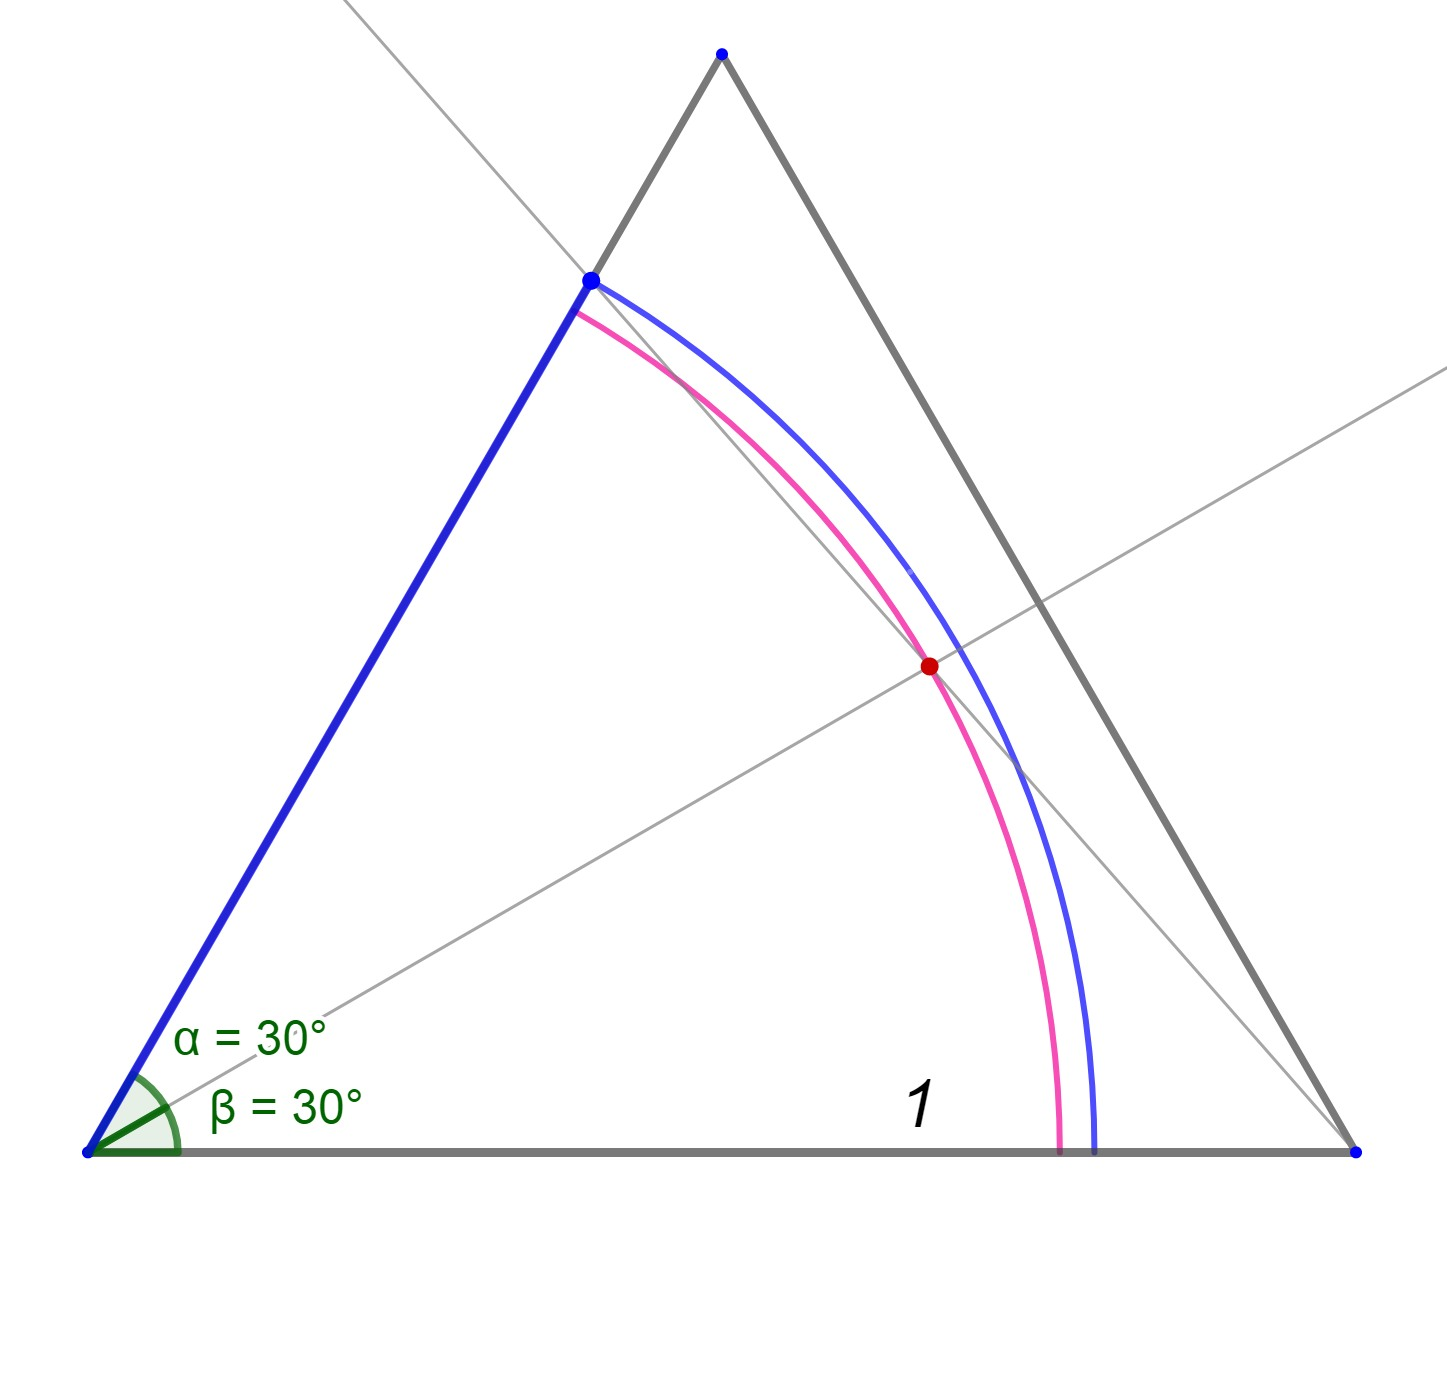
\includegraphics[scale=0.2]{images/ds_tr.jpg}}

\label{logo}
\end{figure}
\textsc{\LARGE Аскарбеков Алмас Серикович }\\[1.5cm]
\begin{center}
	\large {almas@diamondsection.com}\\
	\today
\end{center}
\end{titlepage}


\begin{center}
\section*{Аннотация}
\end{center}
Удвоение куба — классическая античная задача на построение циркулем и линейкой ребра куба, объём которого вдвое больше объёма заданного куба\cite{A}.
\\
Задача сводится к тому, что необходимо построить отрезок равный $\sqrt[3]{2}$ используя циркуль и неразмеченную линейку.
\\
 В 1837 году Пьер Ванцель доказал, что эта задача не может быть решена с помощью циркуля и линейки.
\\
\begin{figure}[h]
	\centering
	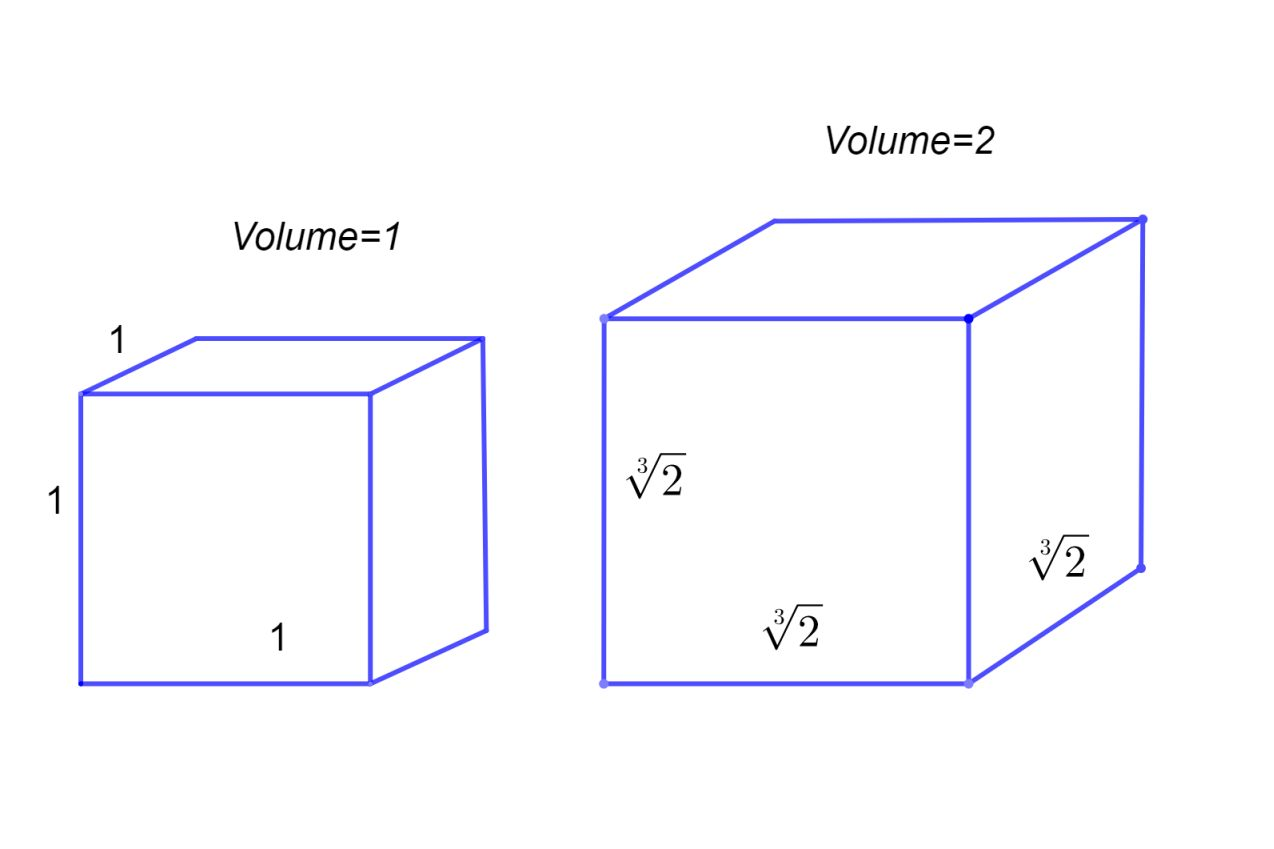
\includegraphics[width=0.7\linewidth]{images/cubes.jpg}
	\label{fig:cubes}
\end{figure}
\begin{figure}[h]
	\centering
	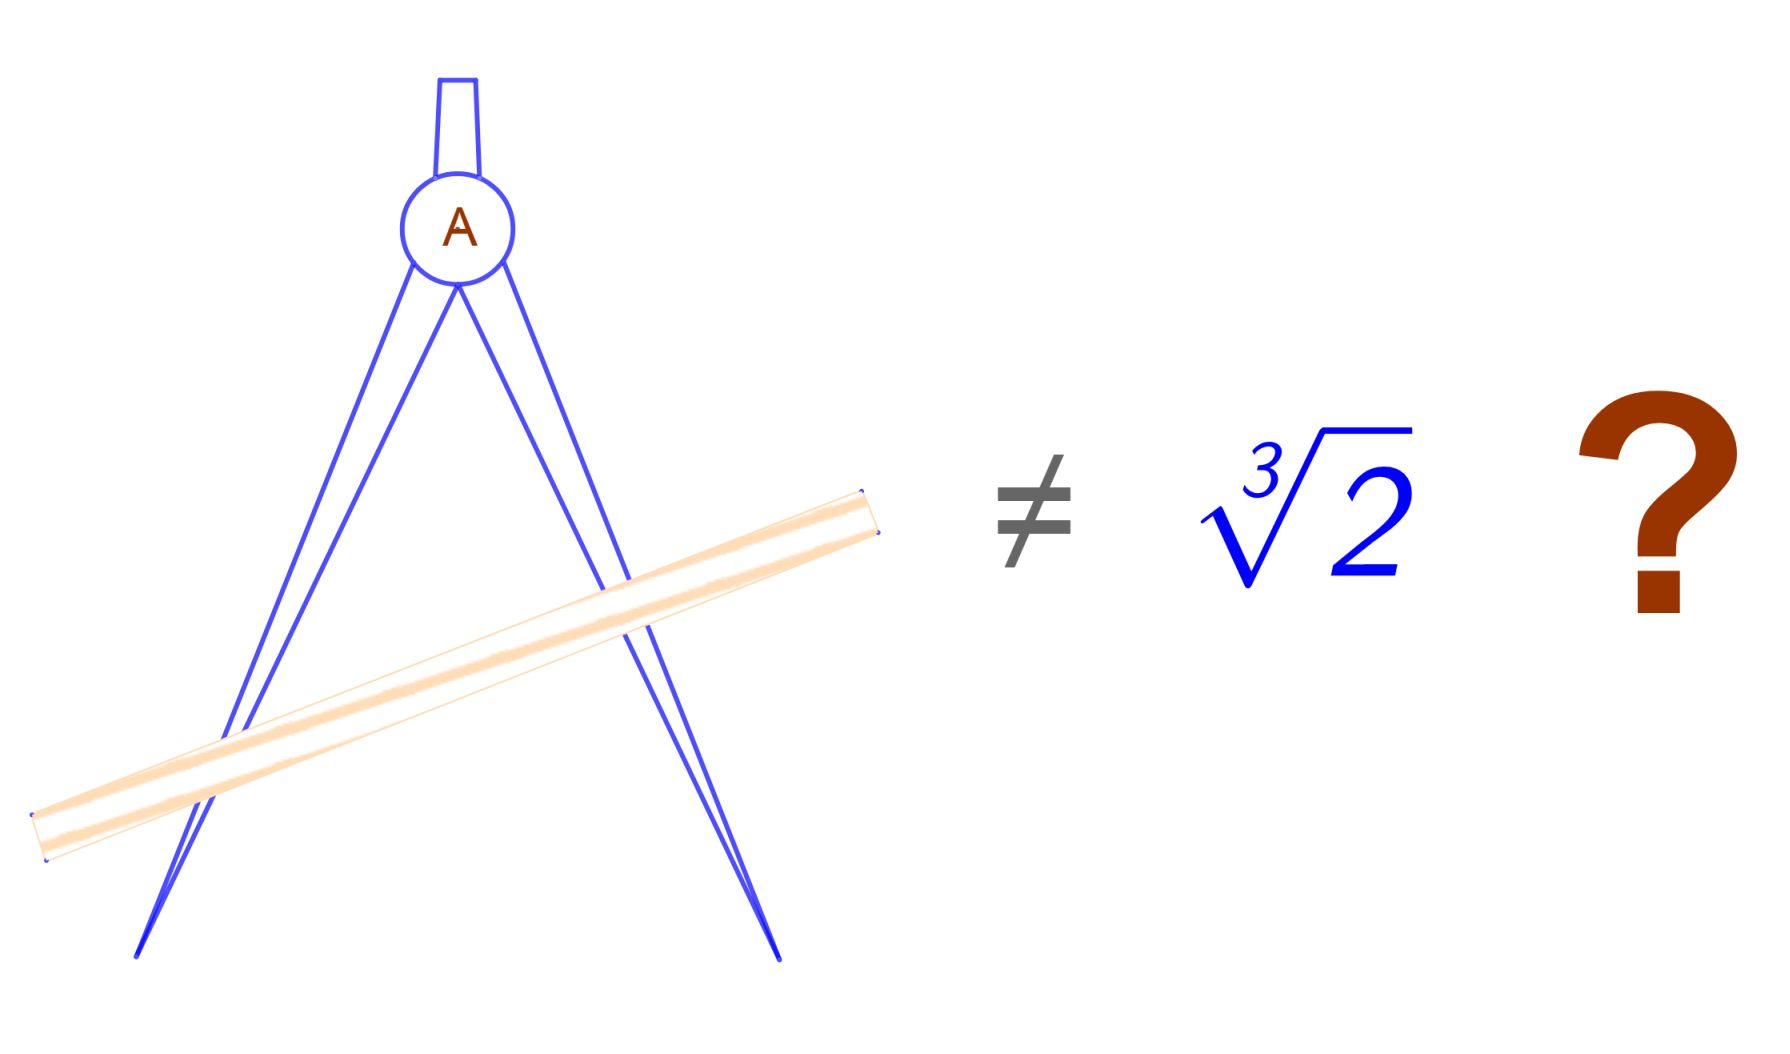
\includegraphics[width=0.8\linewidth]{images/compass.jpg}
	\label{fig:compass}
\end{figure}
\newpage

\tableofcontents


\chapter{}

\section{Построение}
\begin{enumerate}
	\item Построим базовые линии и окружности радиусом $r=1$ как показано на рис 1.1.
\begin{figure}[H]
	\centerline{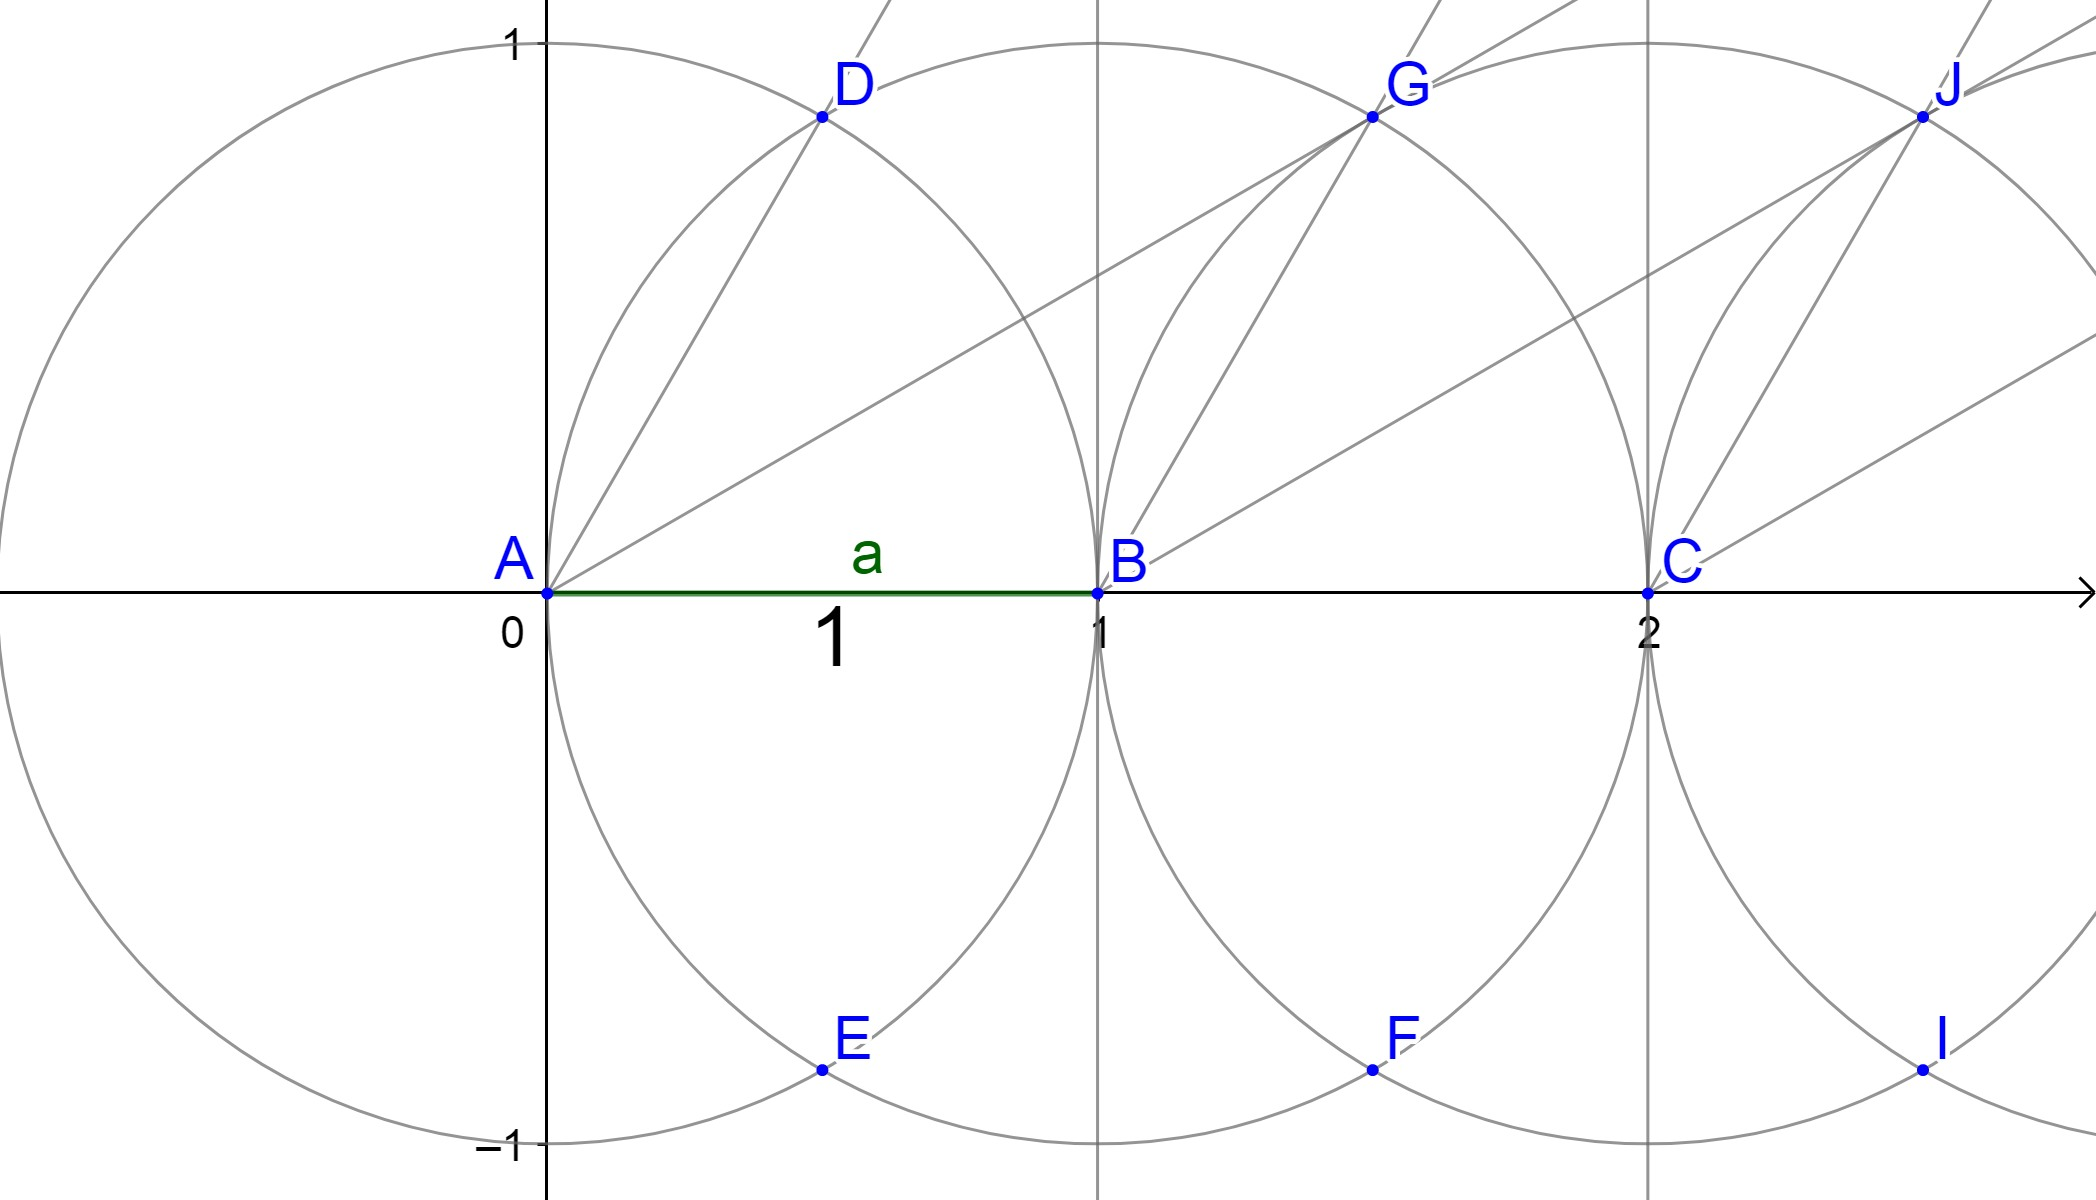
\includegraphics[scale=0.1]{img/basic.jpg}}
	\caption{Базовые окружности}
	\label{fig:basic}
\end{figure}
	
	\item Затем построим прямоугольный треугольник $\triangle ANB$ (Рис. \ref{fig:1_anb}) со стороной $t=0.75$. \\
\begin{figure}[H]
	\centerline{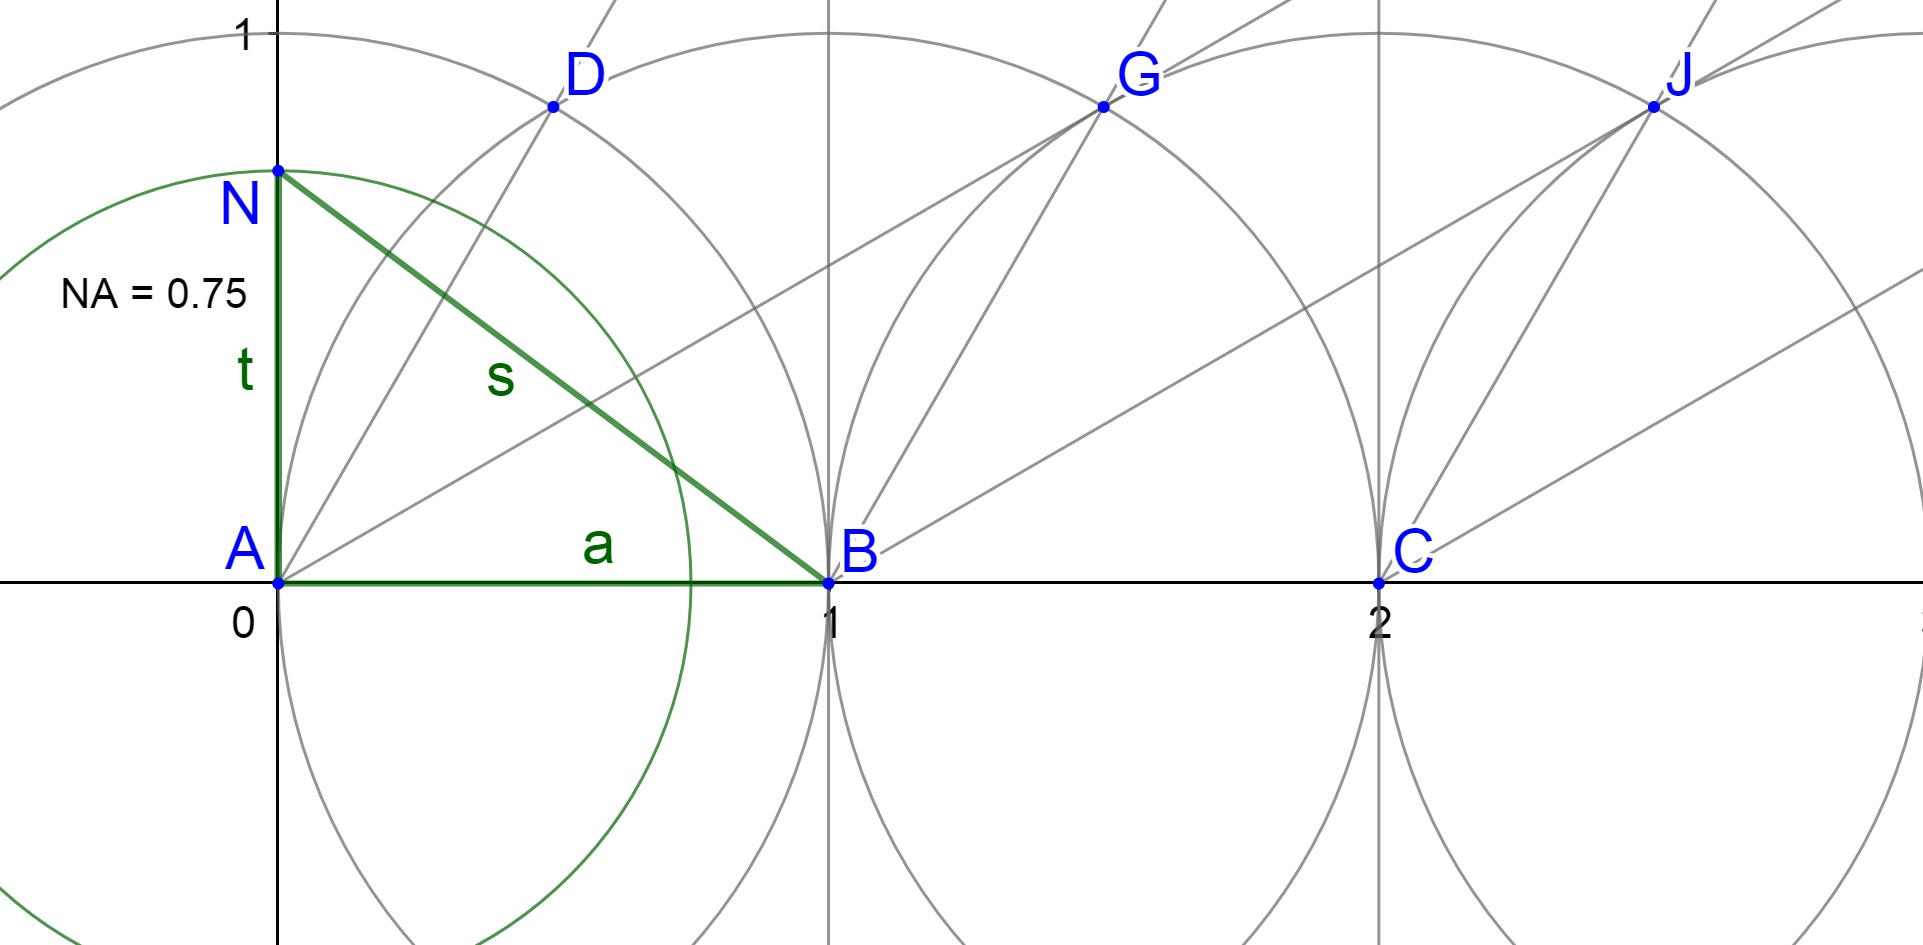
\includegraphics[scale=0.18]{img/1_anb.jpg}}
	\caption{Прямоугольный треугольник}
	\label{fig:1_anb}
\end{figure}	
	Вычислим гипотенузу:
\begin{equation}
s=\overline{NB}=\sqrt{a^{2}+t^{2}}=\sqrt{1^{2}+0.75^{2}}=1.25
\end{equation}
\\
	\item Отсюда отношение катета к гипотенузе:
\begin{equation}
	\dfrac{a}{s}=\cos \angle ABN=\dfrac{1}{1.25}=0.8.
\end{equation}
\\
Что бы построить это отношение проведем линию через точки $N$ и $B$. Мы получим точку $O$ и точку $P$. (см. Рис. \ref{fig:2_second})
\begin{figure}[h]
	\centerline{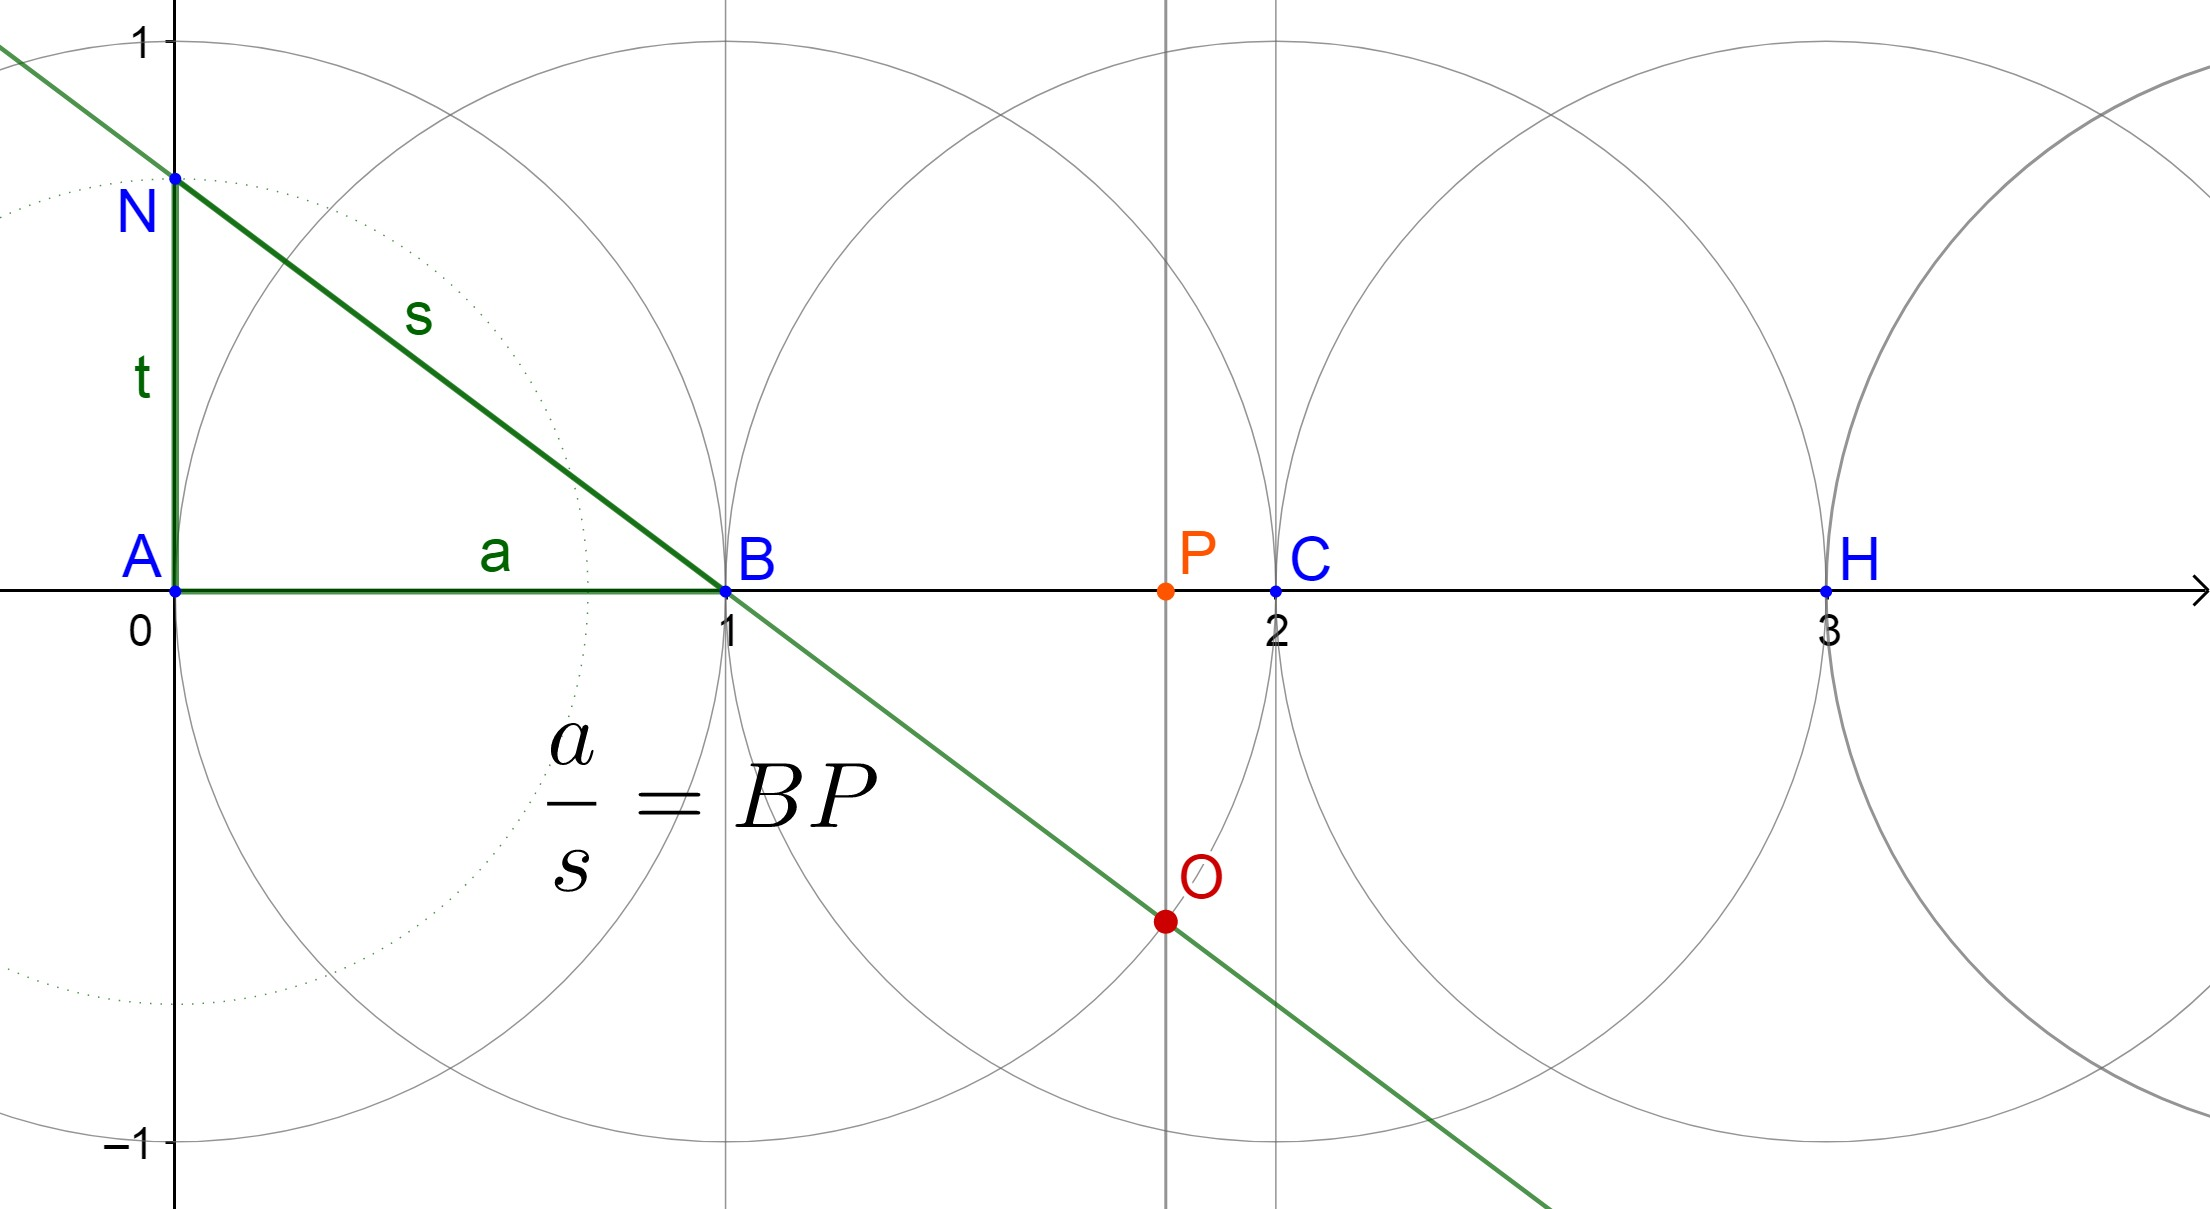
\includegraphics[scale=0.2]{img/anbo.jpg}}
	\caption{}
	\label{fig:2_second}
\end{figure}
\\
	\item Теперь построим окружность с центром $B$ и радиусом = $BP$ (см. Рис \ref{fig:anbop})\\ 
\begin{figure}[h]
	\centerline{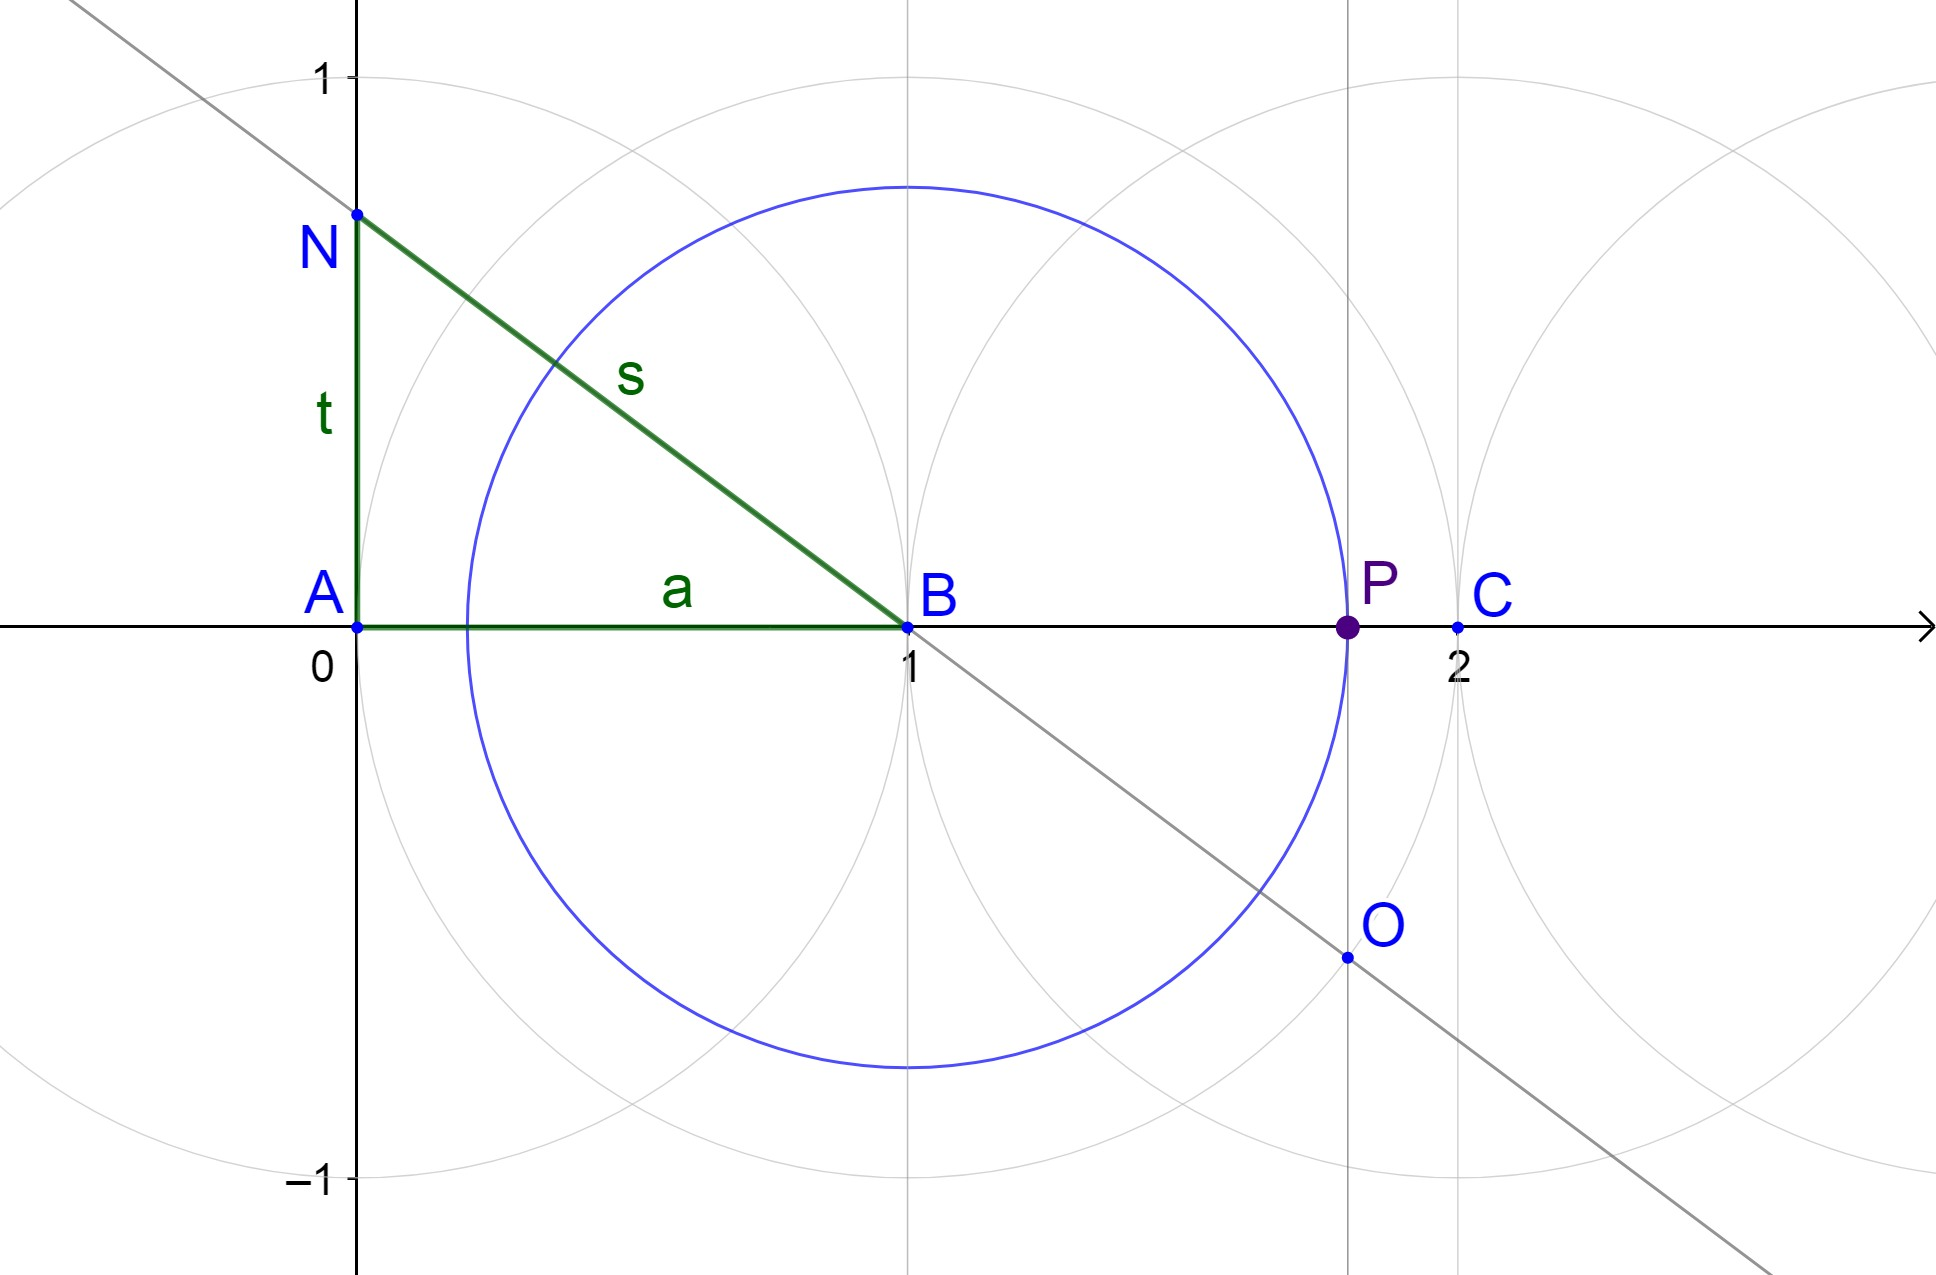
\includegraphics[scale=0.15]{img/anbop.jpg}}
	\caption{}
	\label{fig:anbop}
\end{figure}
\newpage
	\item Затем построим луч из точки $C(2,0)$ через точку $Q$ которая является пересечением окружности и отрезка $\overline{BG}$. (см. Рис. \ref{fig:anbopq}).
\begin{figure}[h]
	\centerline{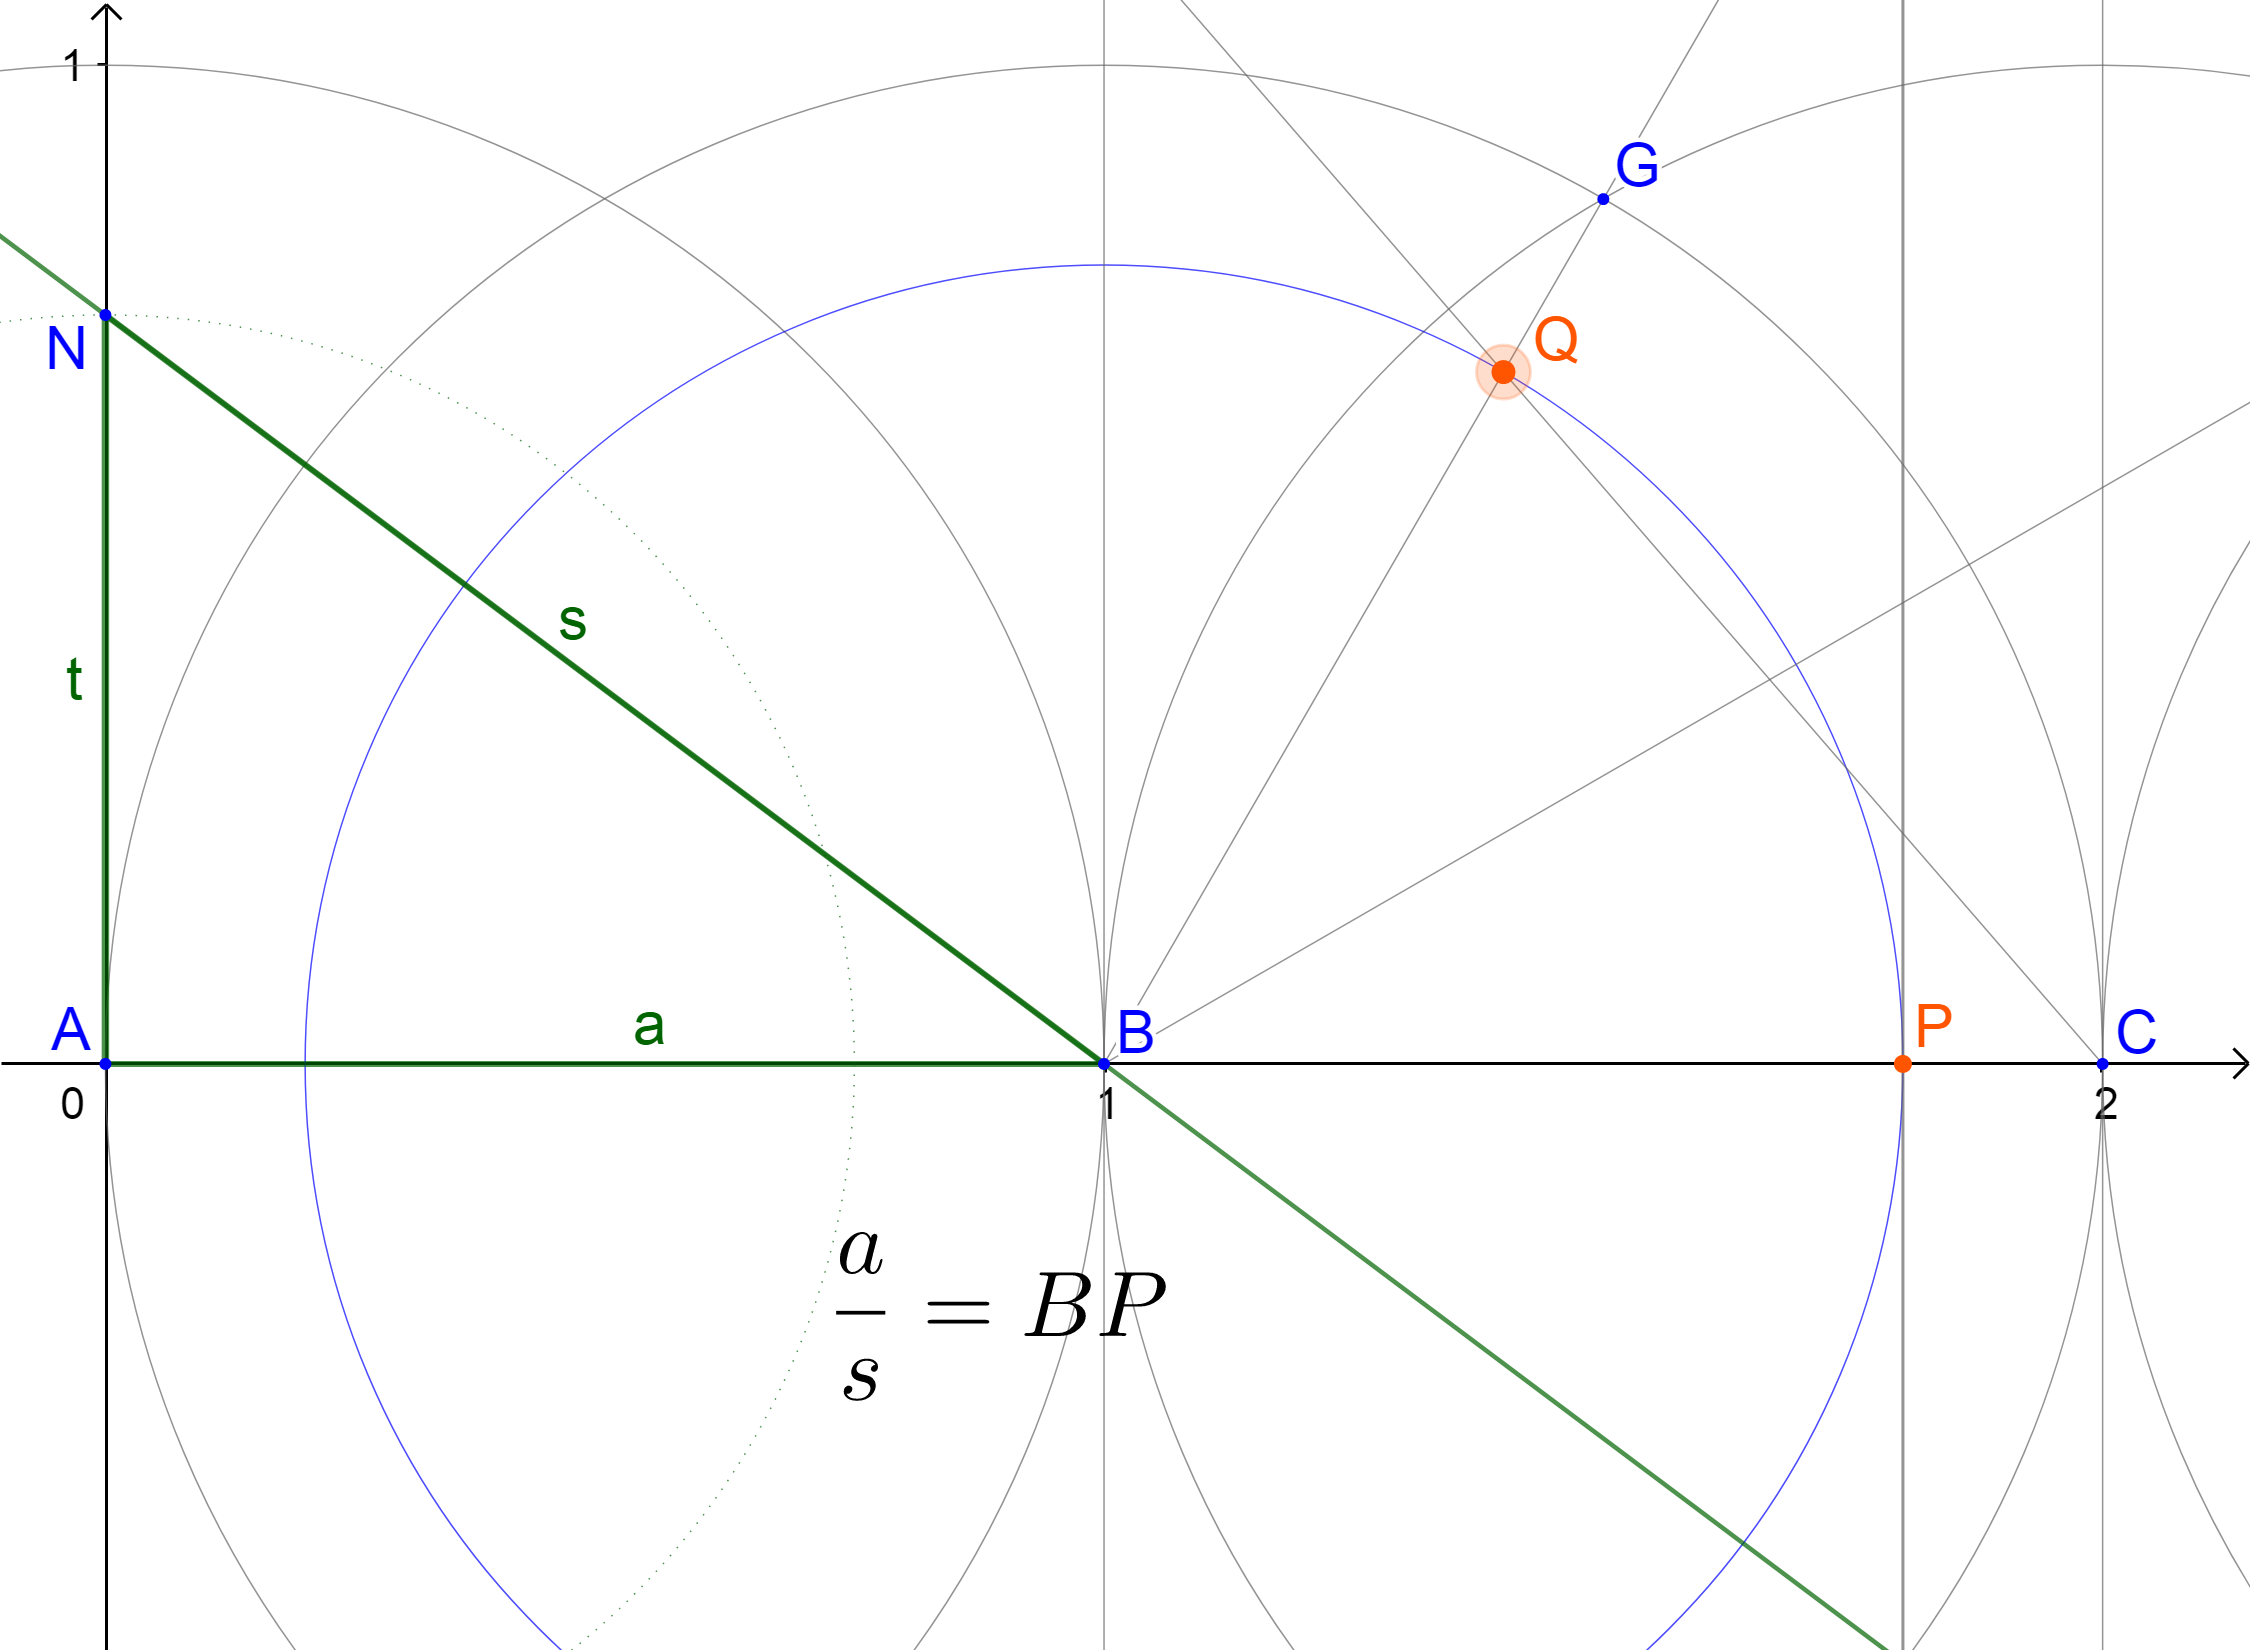
\includegraphics[scale=0.15]{img/anbopQ.png}}
	\caption{}
	\label{fig:anbopq}
\end{figure}
	\item Затем получим точку $R$ как показано на рис. \ref{fig:anbopqr}\\
\begin{figure}[h]
	\centerline{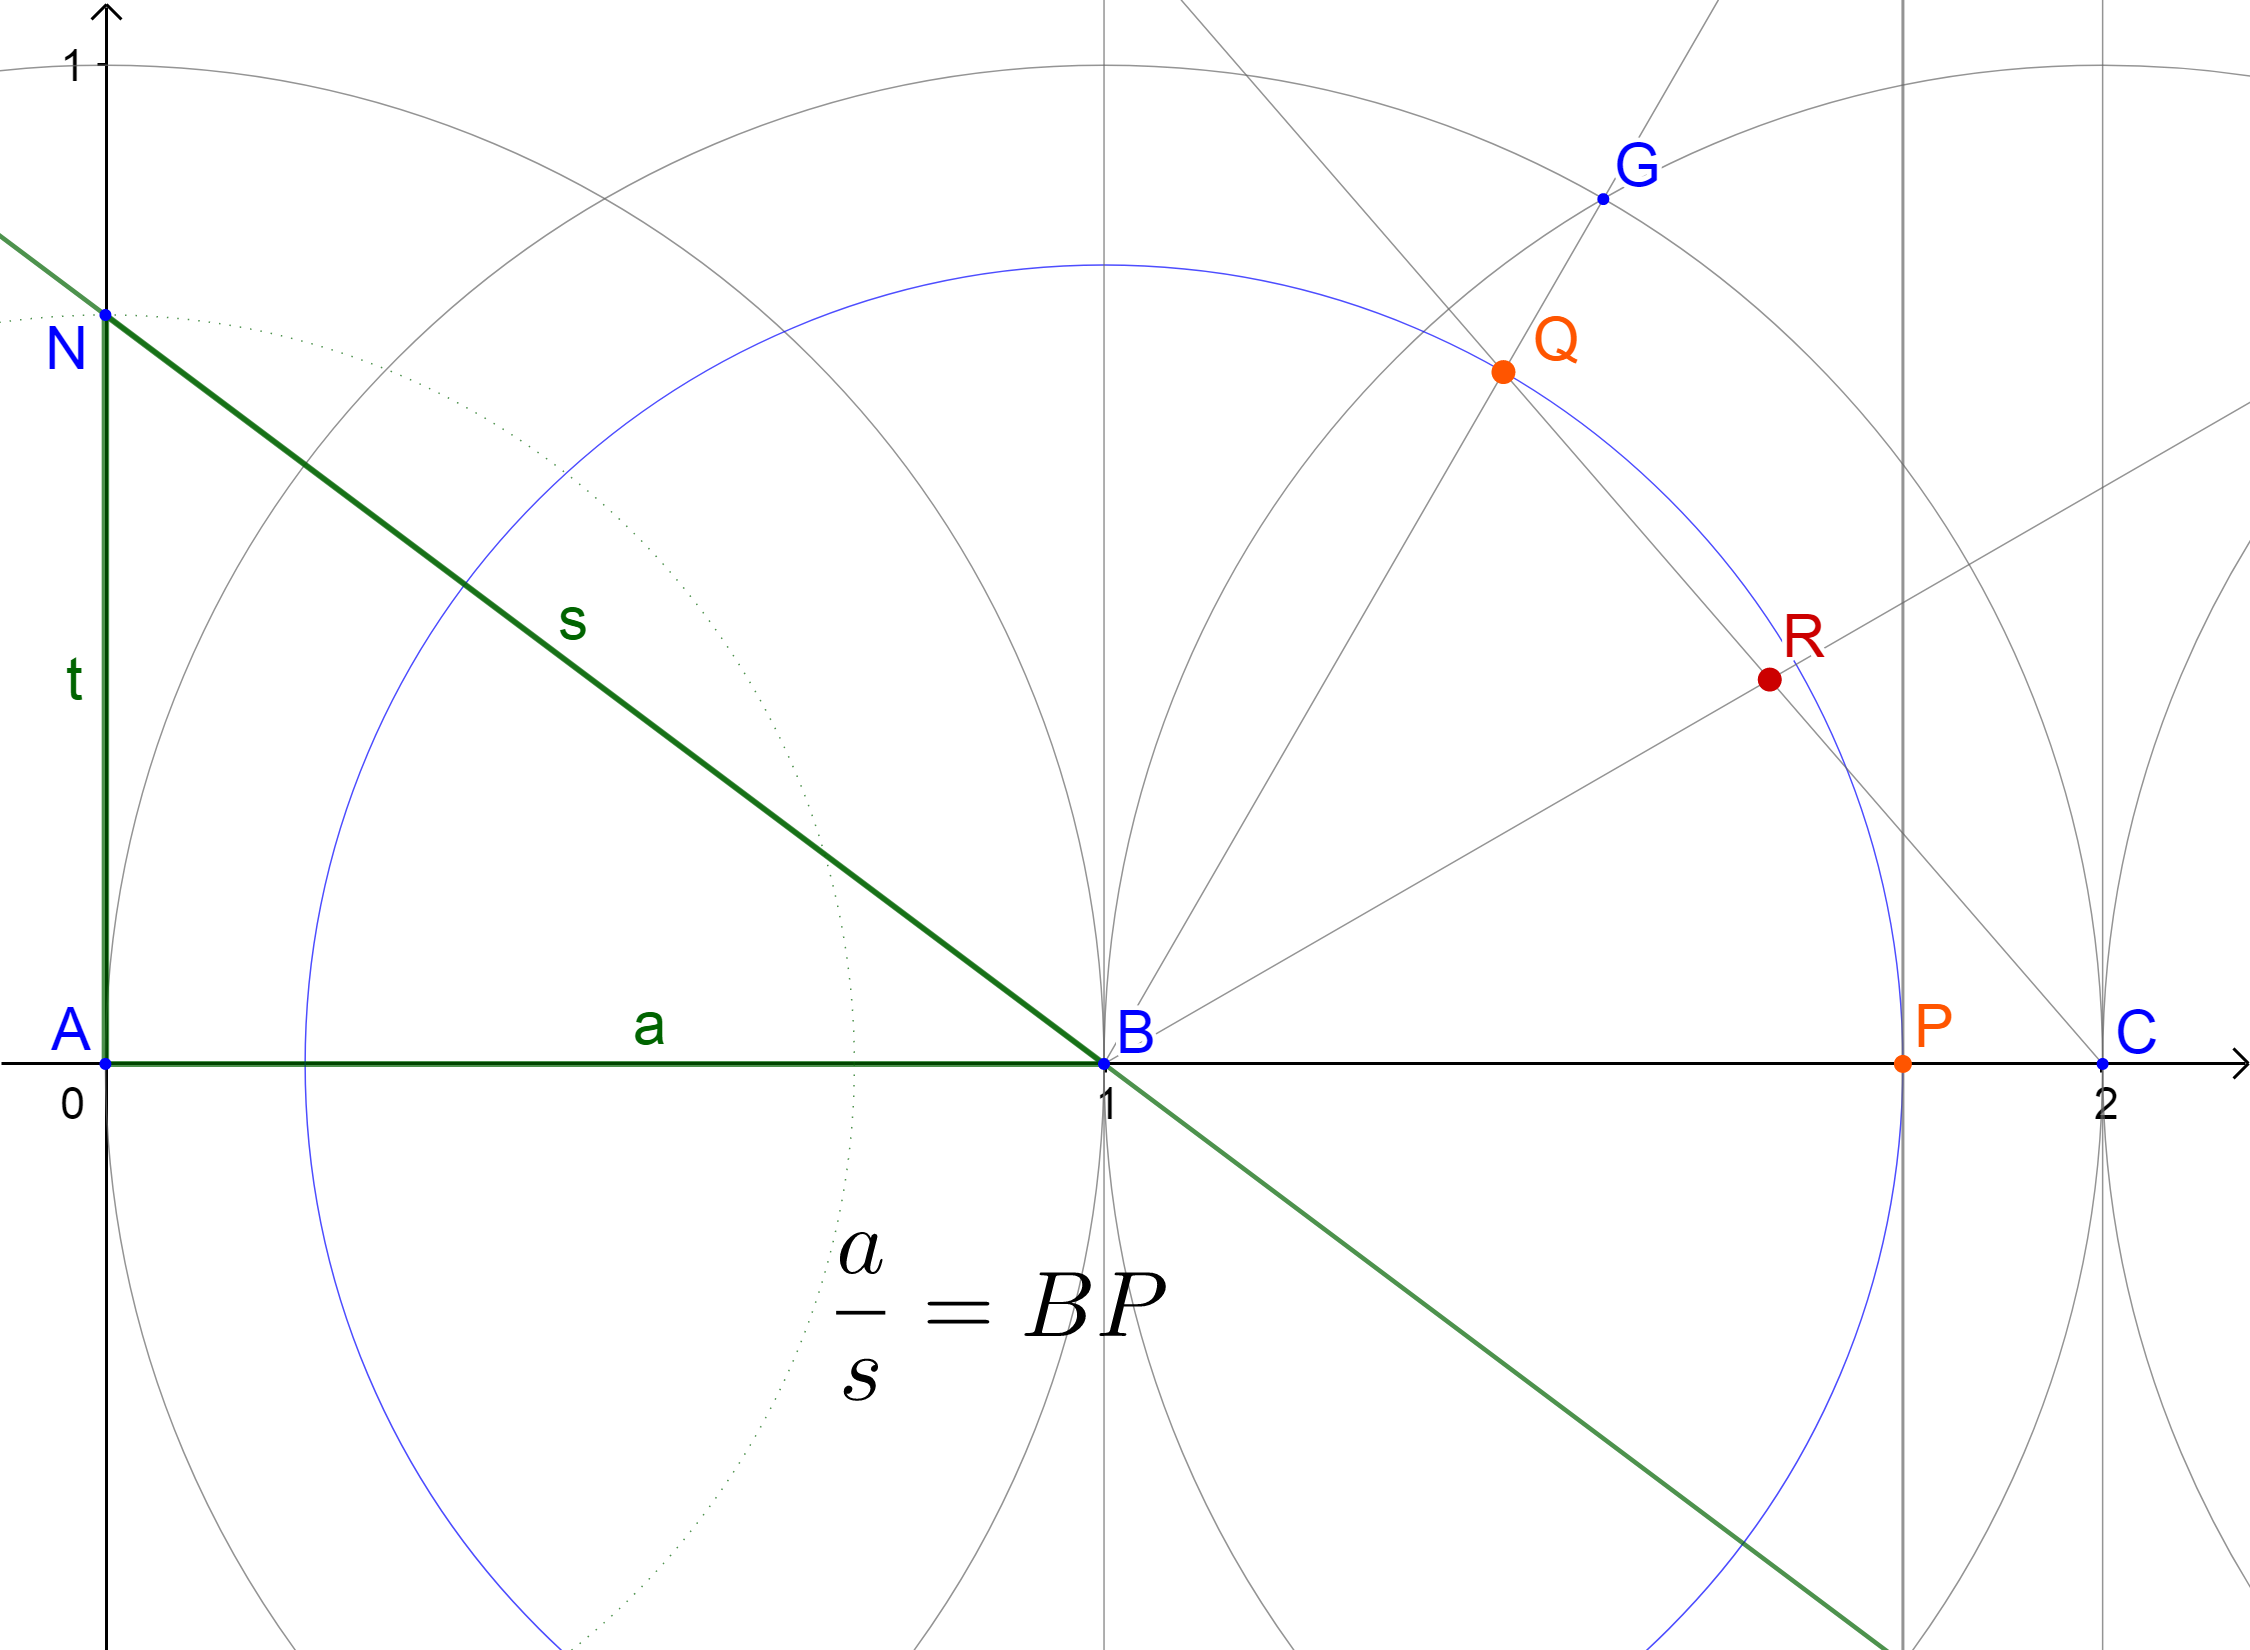
\includegraphics[scale=0.14]{img/anbopqR.png}}
	\caption{}
	\label{fig:anbopqr}
\end{figure}\\
	Отрезок $BR$ это биссектриса $\triangle$ $BQC$  (см. Рис. \ref{fig:bqc})
\newpage
Итак у нас есть треугольник $\triangle$ $BQC$ где $BQ=BP=\dfrac{a}{s}=\cos \angle ABN$.
\begin{figure}[H]
		\centerline{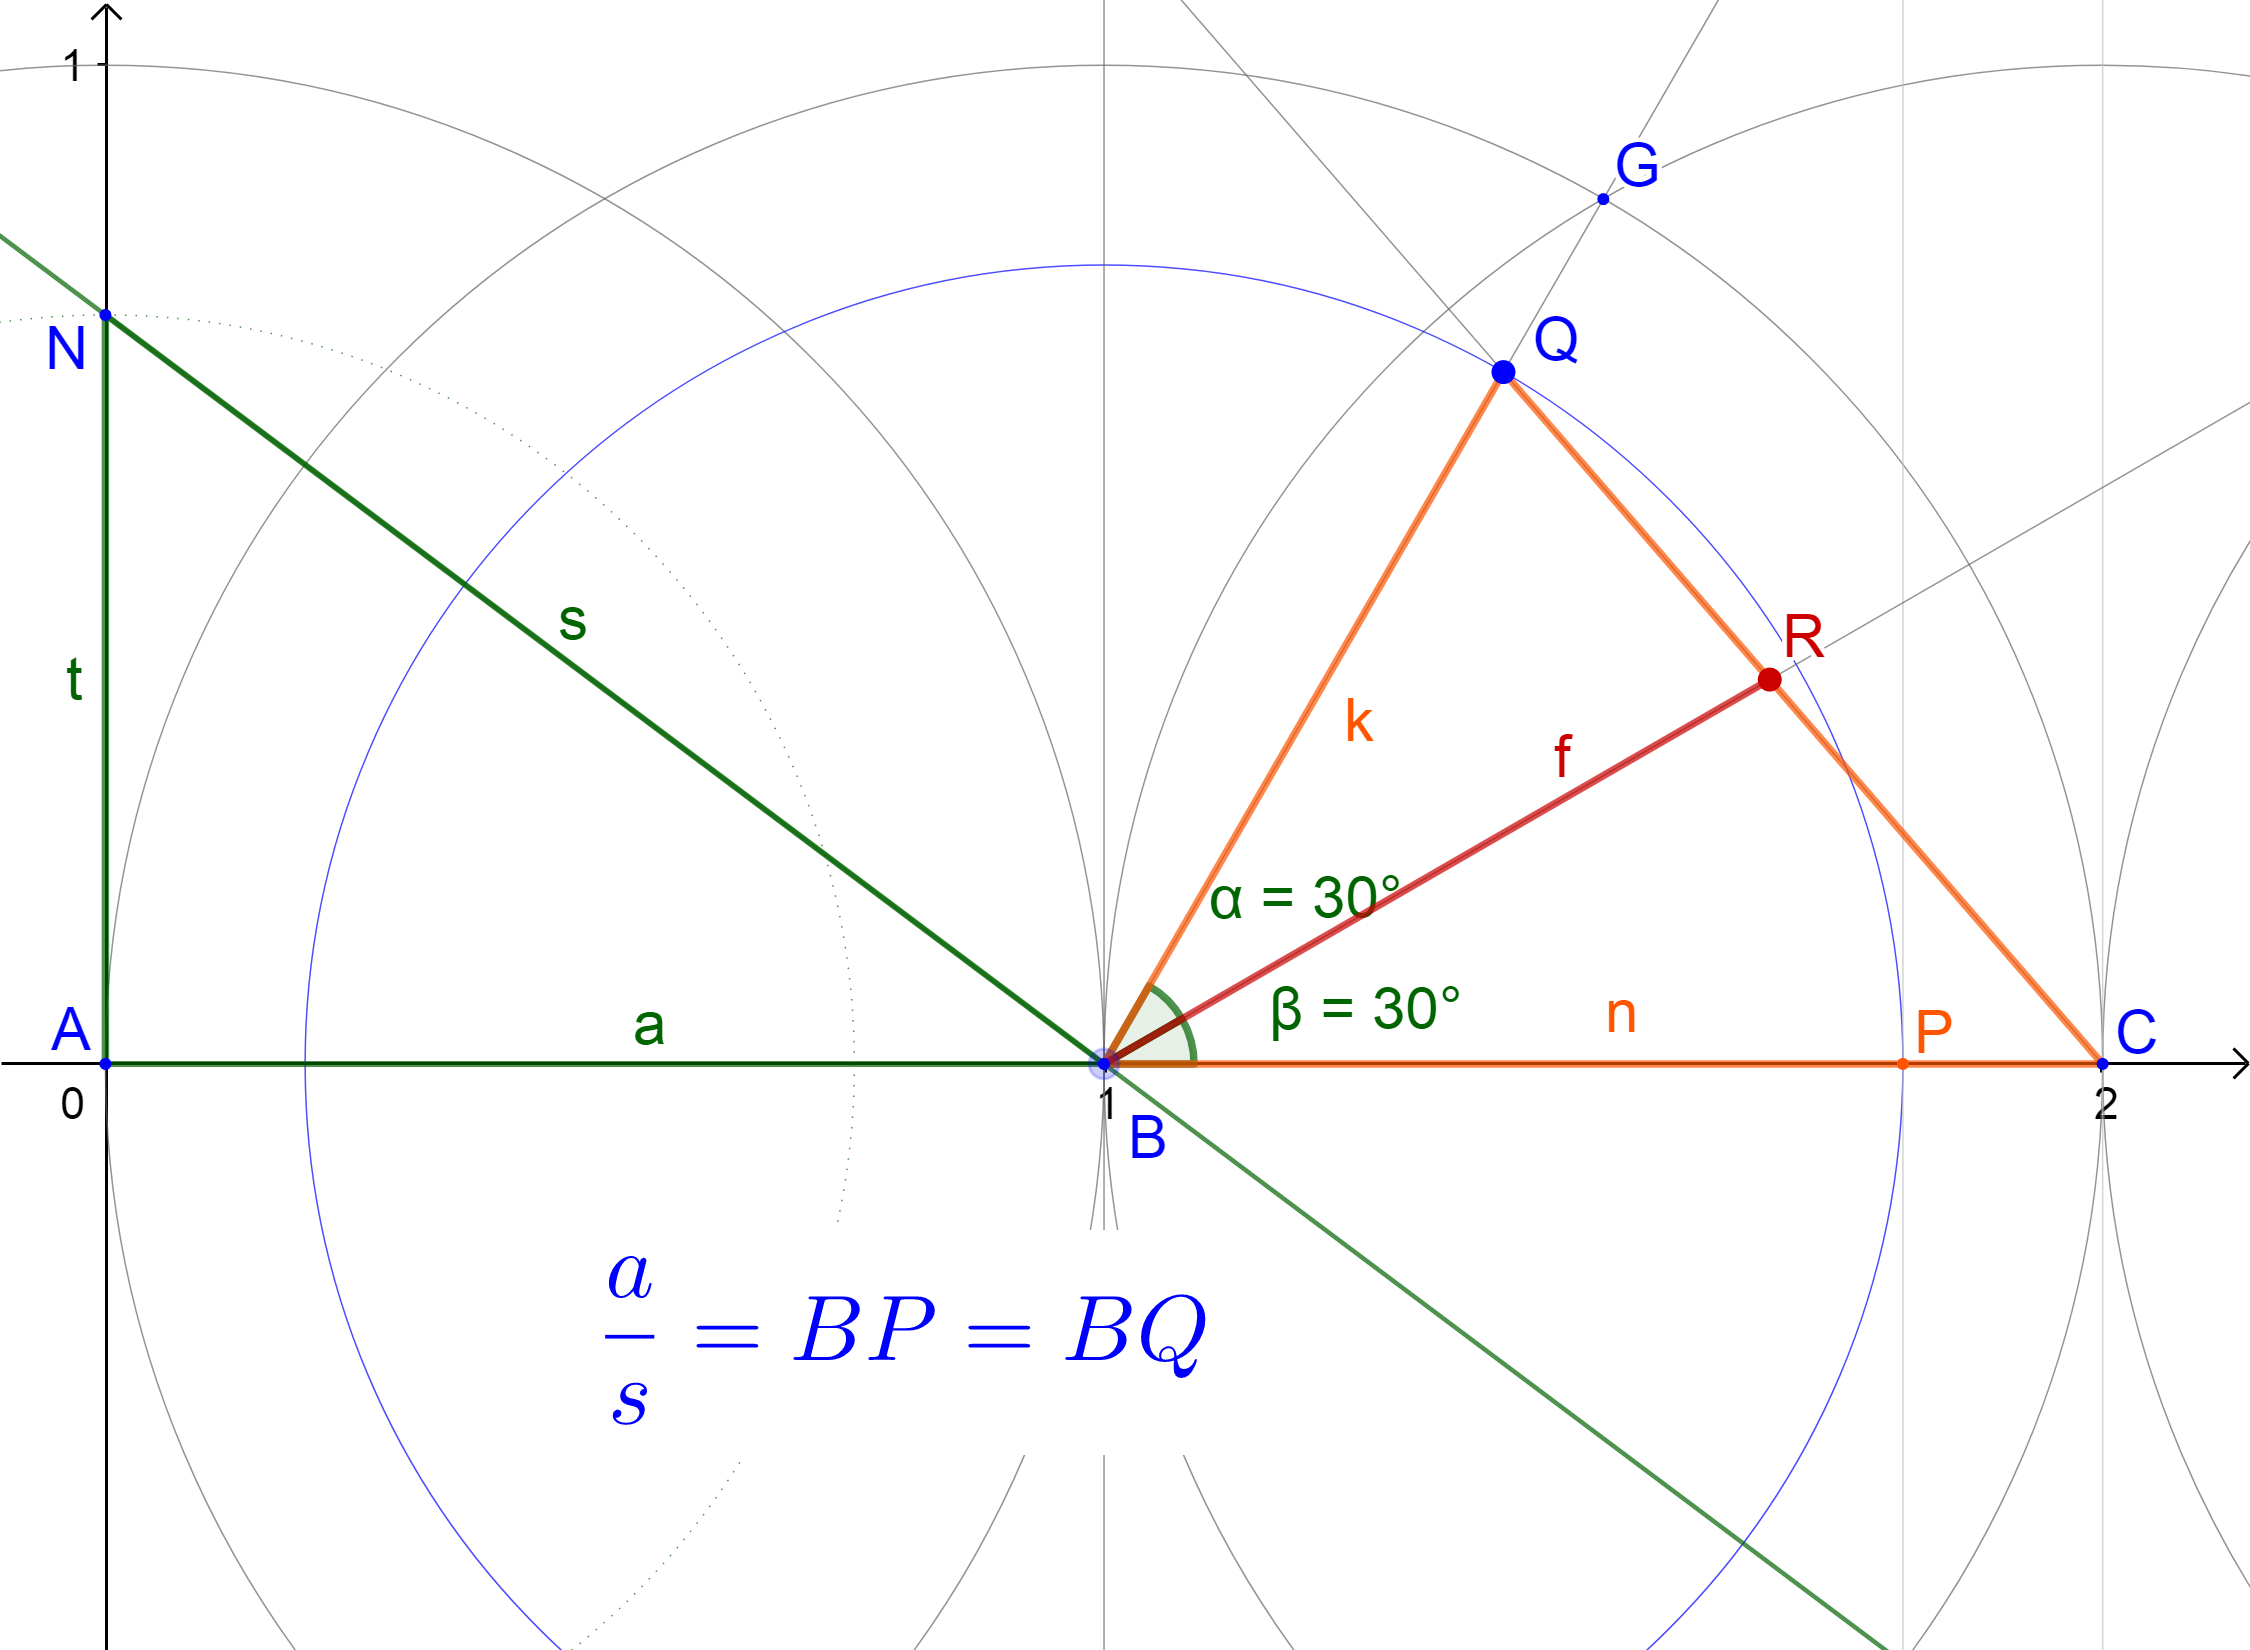
\includegraphics[scale=0.15]{img/BQC.png}}
		\caption{Треугольник $BQC$}
		\label{fig:bqc}
\end{figure}
	\item Вычислим биссектрису $BR$ по формуле длины биссектрисы для угла в 60 градусов:	
\begin{equation}
f=\frac{2nk}{k+n}\times \cos 60\degree = \frac{2nk}{k+n}\times\frac{\sqrt{3}}{2}
\end{equation}\\
	где:  $k=BQ=0.8$; $n=BC=1$; следовательно:
\begin{equation}	
f=\frac{2\times0.8}{1+0.8}\times\frac{\sqrt{3}}{2}\approx 0.769800358919501
\end{equation}
	\item Построим окружность с радиусом = $f$ и центром в точке $B(1,0)$ и получим точку $D$ (см. Рис. \ref{circle})
\begin{figure}[h]
	\centerline{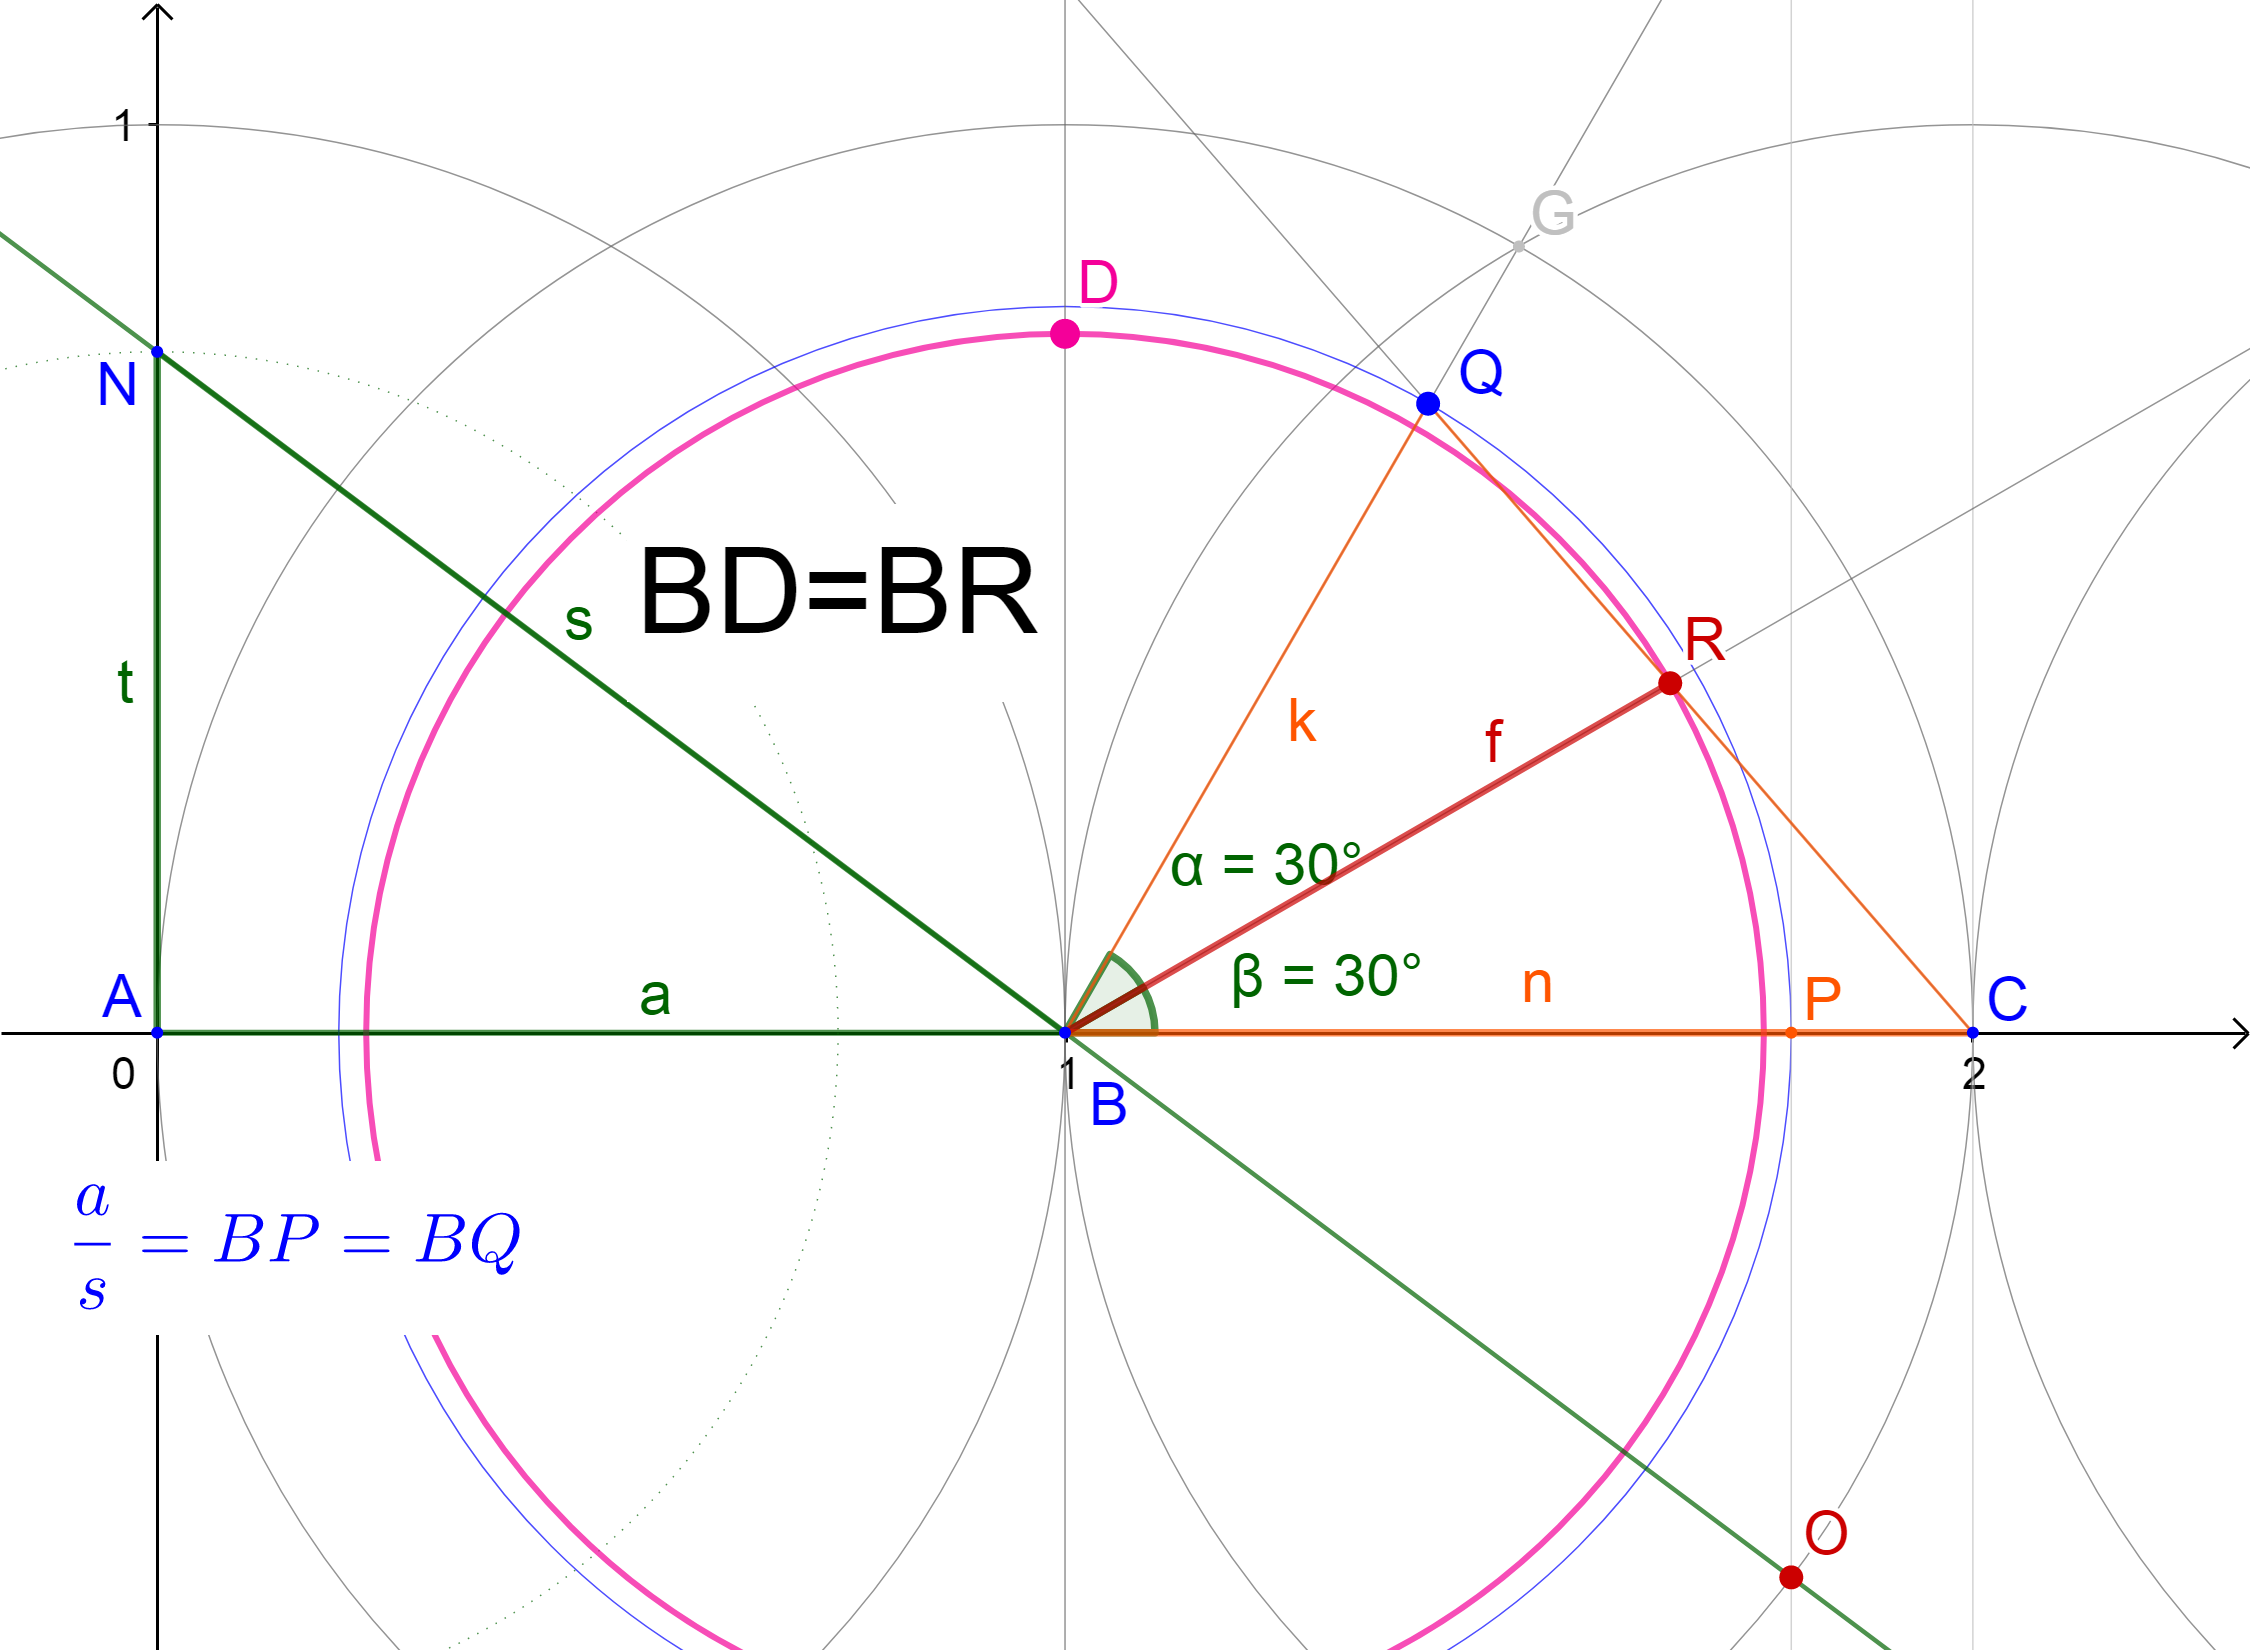
\includegraphics[scale=0.1]{img/bdBR.png}}
	\caption{Окружность где радиус = биссектриса BR}
	\label{circle}
\end{figure} 	
\newpage
	\item Затем снова построим прямоугольный треугольник $\triangle BDC$ как показано на рис. \ref{fig:bdc}.
\begin{figure}[h]
	\centerline{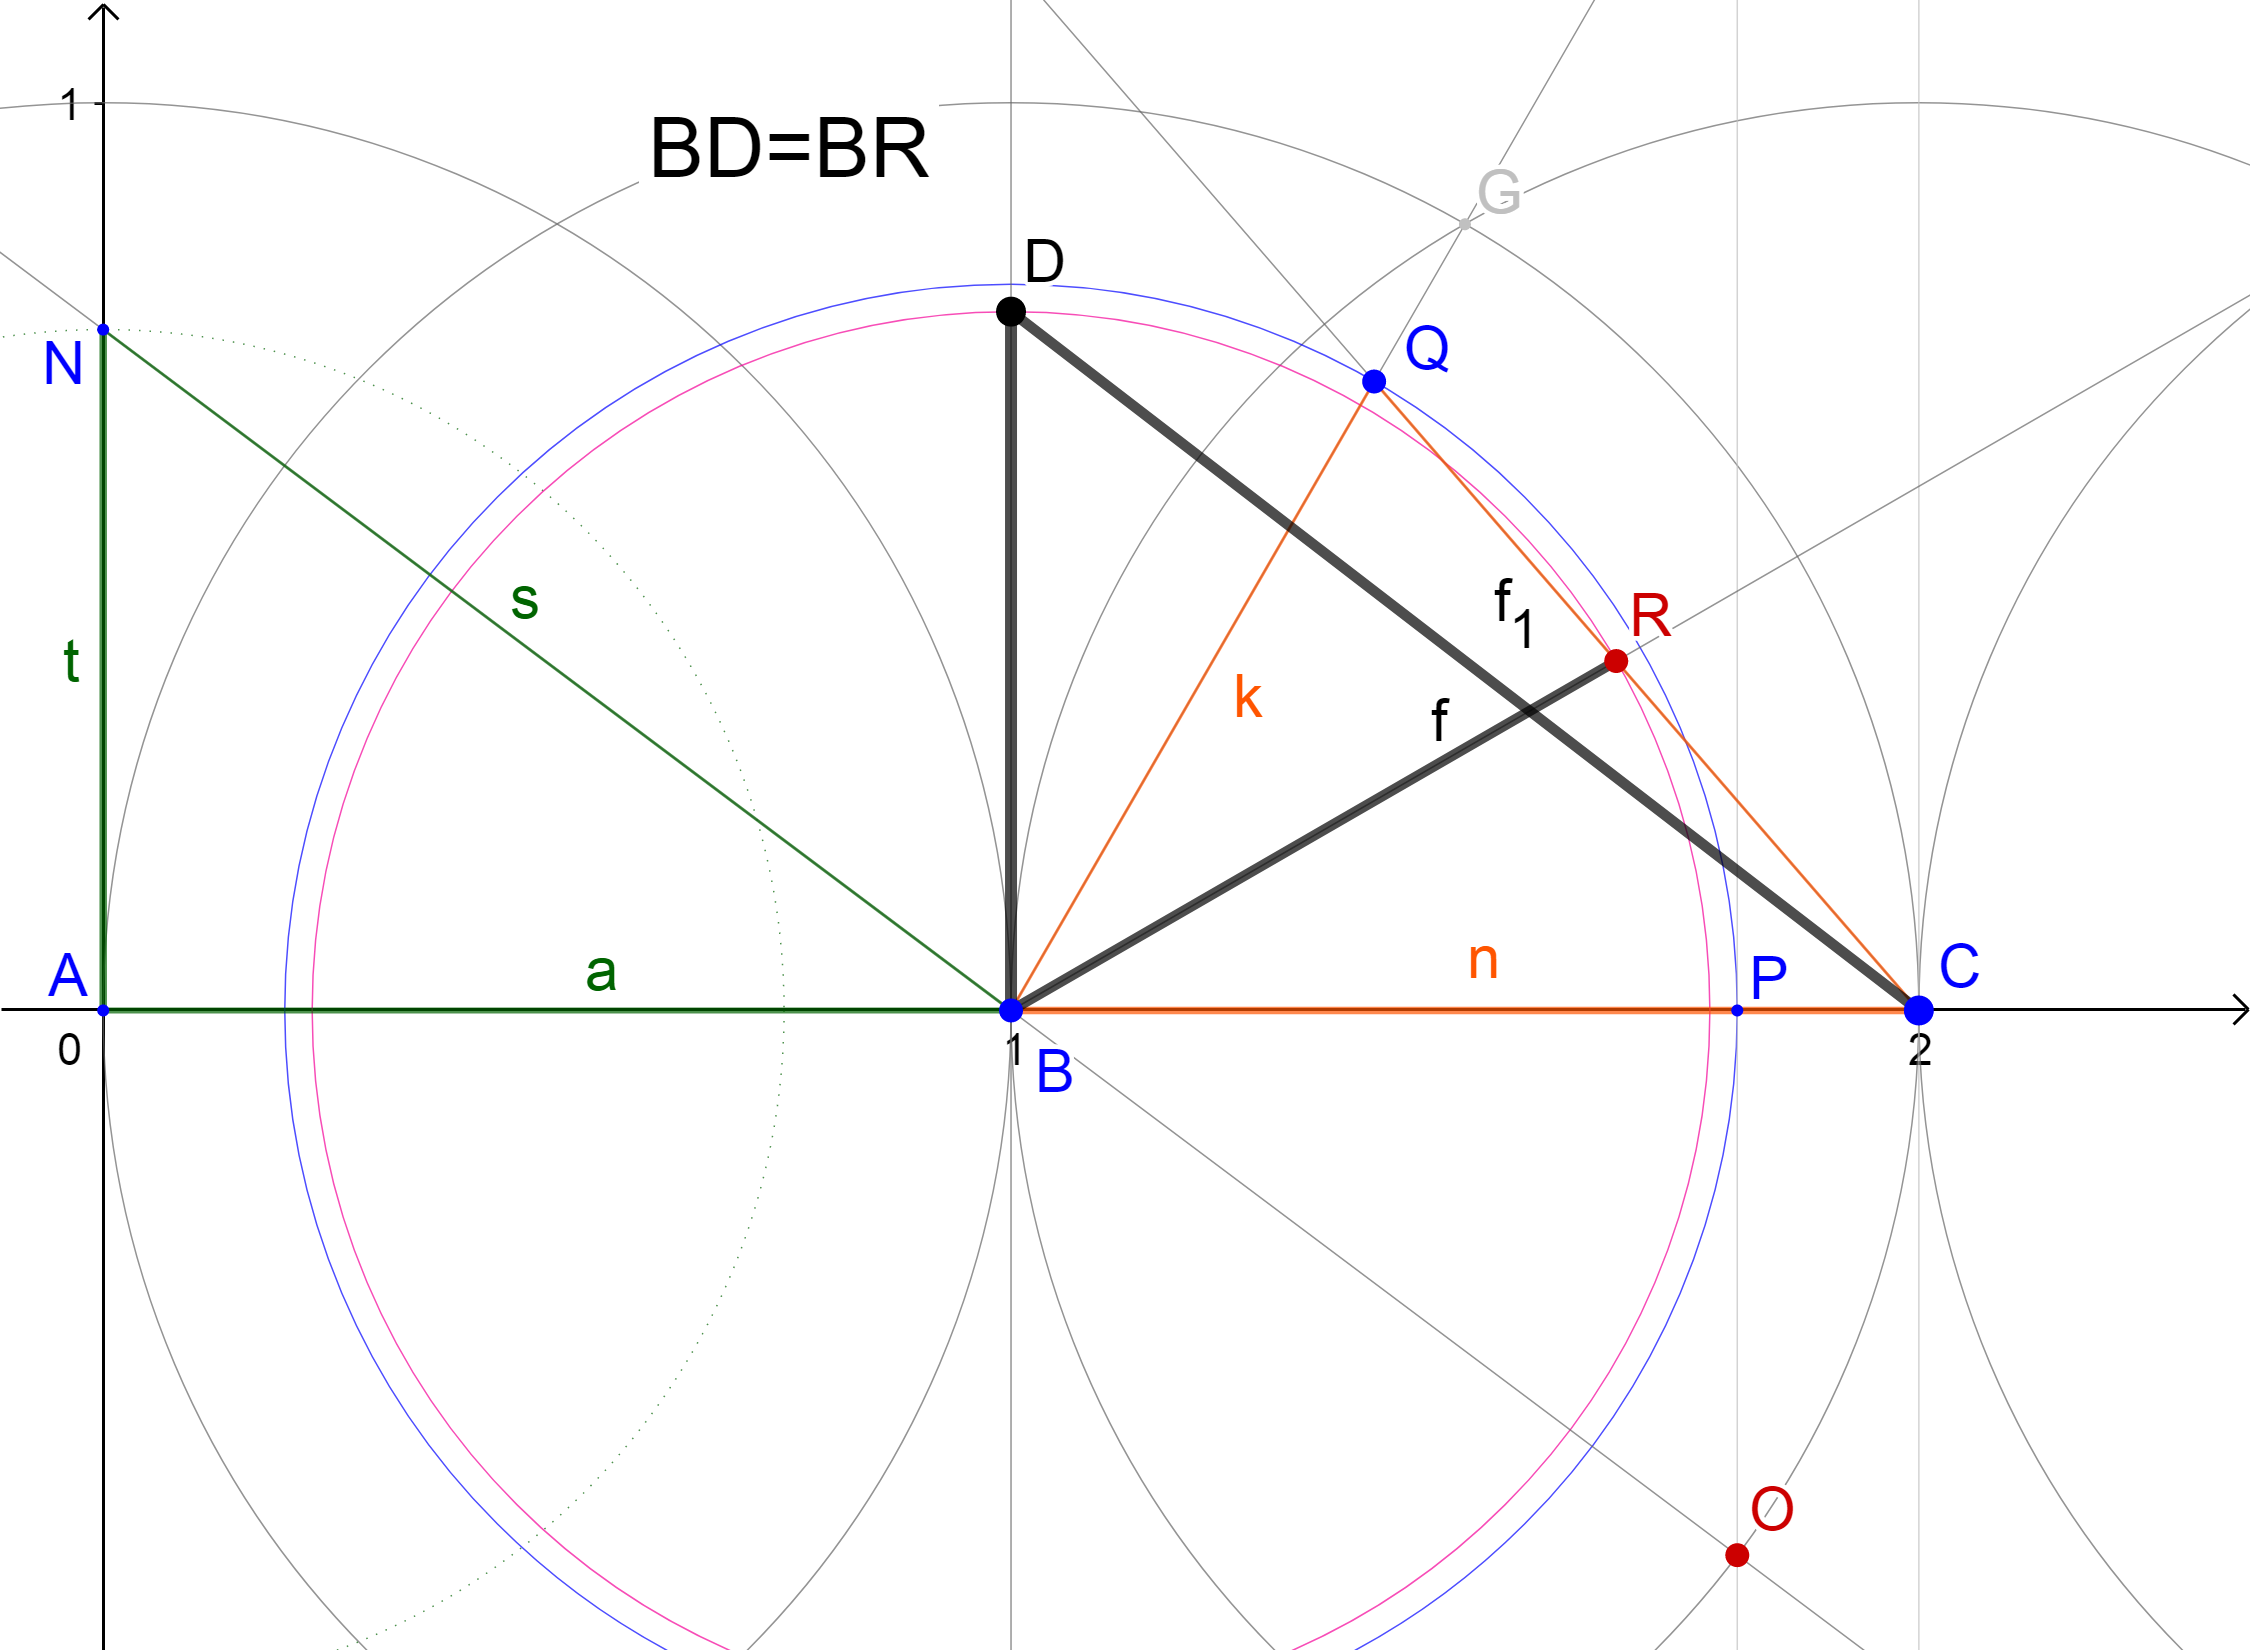
\includegraphics[scale=0.14]{img/BDC.png}}
	\caption{}
	\label{fig:bdc}
\end{figure}\\
Итак мы получили прямоугольный треугольник $\triangle BDC$. Соответсвенно дальше мы повторяем действия: 
\subitem строим значение косинуса
\subitem строим треугольник с углом в 60 градусов
\subitem находим биссектрису
\subitem cтроим прямоугольный треугольник 
\subitemи так снова и снова.\\
Повторяя эти построения, через n-ное построение мы получим $\sqrt[3]{2}$ как длину гипотенузы прямоугольного треугольника. Таким образом длина гипотенузы вычисляемая по приведенной последовательности стремится к $\sqrt[3]{2}$.
\newpage

\end{enumerate}.

\subsection{Доказательство} 


Основная идея похожа на концепцию рекурсии.\\
 
Алгоритм выглядит так:
\begin{enumerate}
\item[1] итерация:
\begin{equation}
\dfrac{1}{\sqrt{a^{2}+t_{0}^{2}}}=t_{1};\ \hspace{5pt} \frac{2\times t_{1}}{1+t_{1}}\times\frac{\sqrt{3}}{2}=t_{2}
\end{equation}
\item[2] итерация
\begin{equation}
 \dfrac{1}{\sqrt{a^{2}+t_{2}^{2}}}=t_{3};\ \hspace{5pt} \frac{2\times t_{3}}{1+t_{3}}\times\frac{\sqrt{3}}{2}=t_{4} \ ...
\end{equation}
\subitem n-ная итерация:
\begin{equation}
\dfrac{1}{\sqrt{a^{2}+t_{n}^{2}}}=t_{n+1};\ \hspace{5pt} \frac{2\times t_{n+1}}{1+t_{n+1}}\times\frac{\sqrt{3}}{2}=t_{n+2} \ \hspace{5pt} ...
\end{equation}
\end{enumerate}
Где $t_{0}=t=0.75$. Здесь мы выбрали 0.75 для удобства, т.к. это значение легко построить циркулем. Однако мы получим $\sqrt[3]{2}$ при любом произвольно выбранном отрезке и результат вычислений будет стремится к $\sqrt[3]{2}$. Точность зависит от количества итераций, соответсвенно мы можем получить результат с любой заданной точностью: $10^{-9}$, $10^{-19}$ или $10^{-29}$ и т.д.
\begin{enumerate}

\item[1] итерация: $\triangle ANB$;  где $AN=t=0.75$; гипотенуза и косинус соответсвенно:
\begin{equation}
 NB=\sqrt{1^{2}+0.75^{2}}=1.25
 \end{equation}

\begin{equation}
\cos=\dfrac{1}{1.25}=0.8
\end{equation}

биссектриса:
\begin{equation}
 \frac{2\times0.8}{1+0.8}\times\frac{\sqrt{3}}{2}\approx 0.769800358919501
\end{equation}
\\
гипотенуза:
\begin{equation}
\sqrt{1^{2}+0,769800358919501^{2}}\approx 1,261979632400061
\end{equation}
\item[2] итерация:
%\textit{2-nd iteration} 
\begin{equation}
\cos=\dfrac{1}{1,261979632400061}\approx0,792405815693061
\end{equation}
биссектриса:
\begin{equation}
\frac{2\times 0.792405815693061}{1+0.792405815693061}\times\frac{\sqrt{3}}{2}\approx 0.765723432147395
\end{equation}
\\
гипотенуза:
\begin{equation}
\sqrt{1^{2}+0.765723432147395^{2}}\approx 1.259496873572772
\end{equation}
\end{enumerate}
\newpage
Я вычислил значения для 20-ти итераций, затем проанализировал данные. В таблице \ref{iterations and values} первая колонка содержит значения катета, во второй колонке значения гипотенузы.
\\
\vspace{10pt}
%The last value of the hypotenuse is \textbf{1.259921049894873}, which is equal to  $\sqrt[3]{2}$ with an accuracy of $10^{-15}$. \\


\begin{tabular}{|c|c|c|} \hline
\centering
\textbf{iteration}	& \textbf{катет=биссектриса} & \textbf{гипотенуза}\\	\hline
	$1$         & $0.769800358919501$ & $1.261979632400061$ \\ \hline
	$2$         & $0.765723432147395$ & $1.259496873572772$ \\ \hline
	$3$         & $0.766564817073686$ & $1.260008578849848$ \\ \hline
	$4$         & $0.766391253457252$ & $1.259902993637120$ \\ \hline
	$5$         & $0.766427060119643$ & $1.259924774930487$ \\ \hline
	$6$         & $0.766419673248706$ & $1.259920281423651$ \\ \hline
	$7$         & $0.766421197157344$ & $1.259921208430153$ \\ \hline
	$8$         & $0.766420882775838$ & $1.259921017189131$ \\ \hline
	$9$        & $0.76642094763258$ & $1.259921056642051$ \\ \hline
	$10$        & $0.766420934252668$ & $1.259921048502934$ \\ \hline
	$11$        & $0.766420937012937$ & $1.259921050182029$ \\ \hline
	$12$        & $0.766420936443495$ & $1.259921049835633$ \\ \hline
	$13$        & $0.76642093656097$ & $1.259921049907094$ \\ \hline
	$14$        & $0.766420936536735$ & $1.259921049892352$ \\ \hline
	$15$        & $0.766420936541735$ & $1.259921049895393$ \\ \hline
	$16$        & $0.766420936540704$ & $1.259921049894766$ \\ \hline
	$17$        & $0.766420936540916$ & $1.259921049894895$ \\ \hline
	$18$        & $0.766420936540872$ & $1.259921049894869$ \\ \hline
	$19$        & $0.766420936540881$ & $1.259921049894874$ \\ \hline
	$20$        & $0.766420936540879$ & $1.259921049894873$ \\ \hline

\end{tabular} 
\begin{table}[H] %due to the strange bug with table, here the trick; so that we can see a label and a caption for the table above 
	\caption {Значения для 20-ти треугольников}
	\label{iterations and values}
\end{table}

После анализа данных\footnote{Значения гипотенузы} и применения модели регрессии, получилось кубическое уравнение:
\begin{equation}
y=0.375x^{3}-0.5x^{2}+1.25x
\end{equation}
\begin{figure}[h]
	\centering
	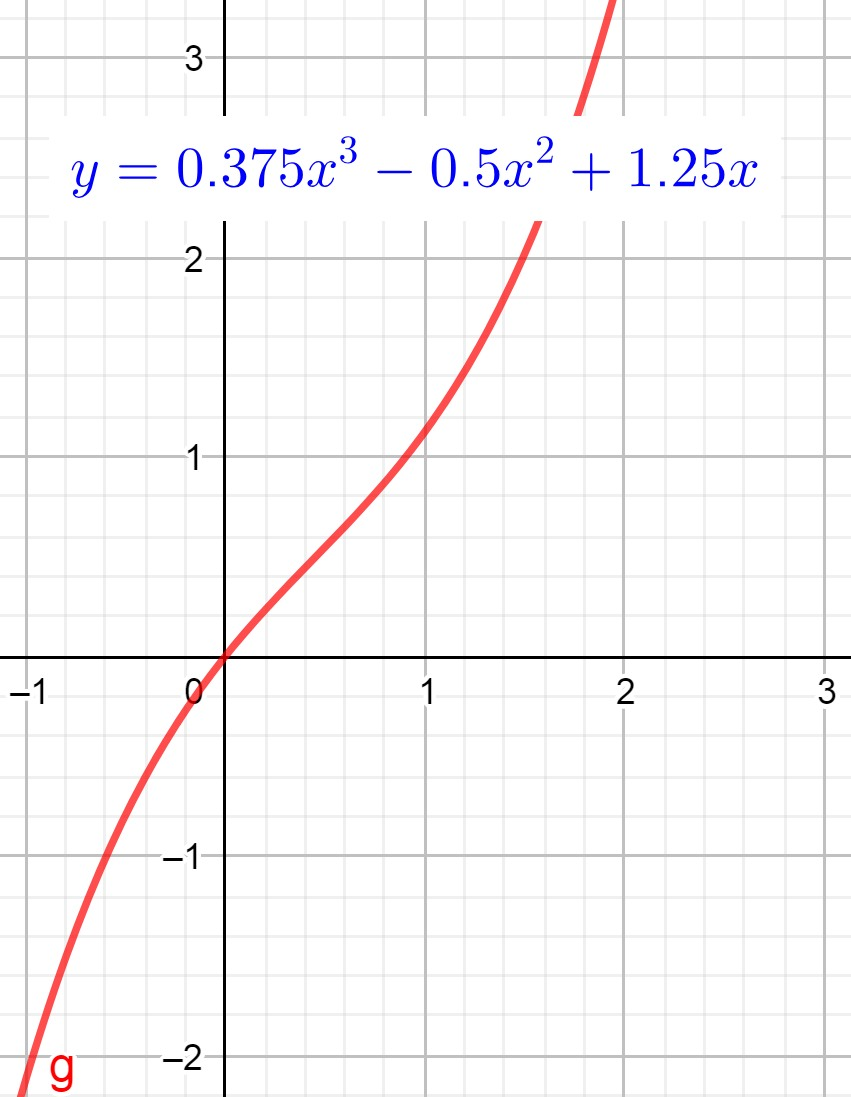
\includegraphics[width=0.25\linewidth]{images/g_x_func.jpg}
	\caption{Функция}
	\label{fig:function}
\end{figure}\\
\newpage
Нас интересует значение гипотенузы на 20-ой строке (Таблица \ref{iterations and values}) и значение медианы (см. Статистику на рис. \ref{fig:data}).

\begin{center}
	Итак это значение = \textbf{1.259921049894873} = $\sqrt[3]{2}$ с точностью до $10^{-15}$.
\end{center}
\vspace{5pt}
\begin{center}
Истинное значение $\sqrt[3]{2}$ = \textbf{1.25992104989487316…} с точностью до $10^{-17}$.\cite{B}
\end{center}
\vspace{5pt}

Здесь стоит отметить что мы получили результат с точностью до $10^{-15}$ потому что в таблице были использованы данные округленные до $10^{-15}$, следовательно если мы будем использовать данные округленные до $10^{-25}$ в итоге мы получим значение $\sqrt[3]{2}$ c точностью до $10^{-25}$. Статистика и график \footnote{График доступен по ссылке:  https://www.geogebra.org/classic/TpwsEbx2} на рис. \ref{fig:plot} наглядно показывают  что результат стремится к $\sqrt[3]{2}$.
\\
\begin{figure}[h]
	\centering
	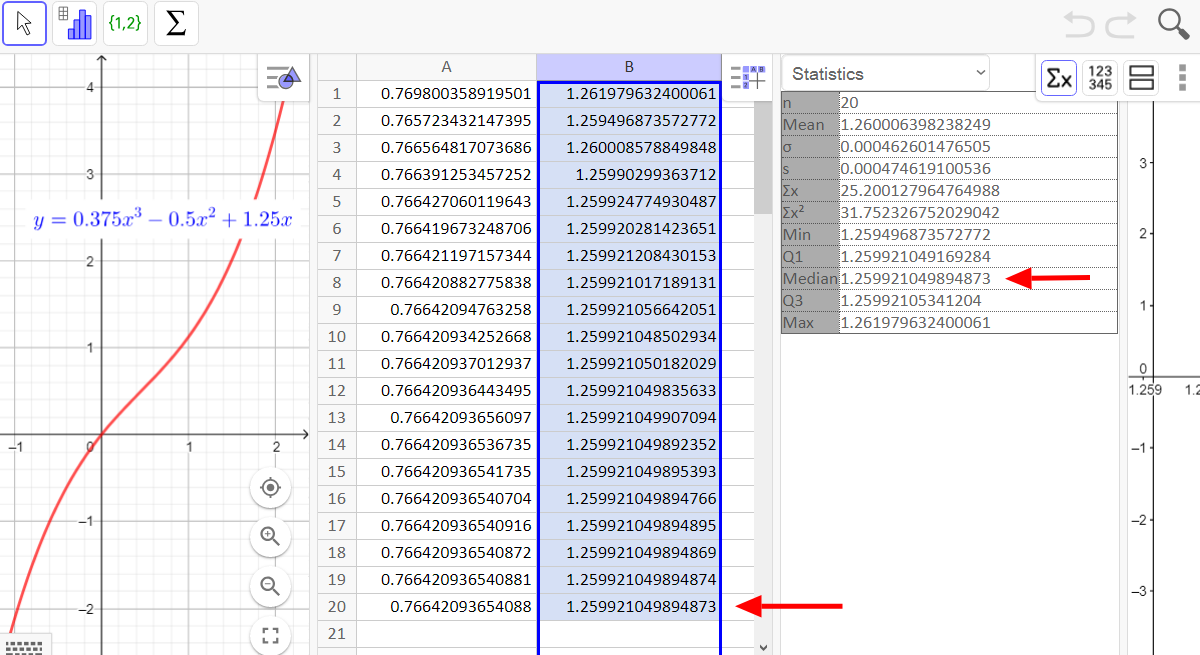
\includegraphics[width=0.88\linewidth]{images/Table_arrow.png}
	\caption{Анализ данных и статистика}
	\label{fig:data}
\end{figure}
\begin{figure}[h]
	\centering
	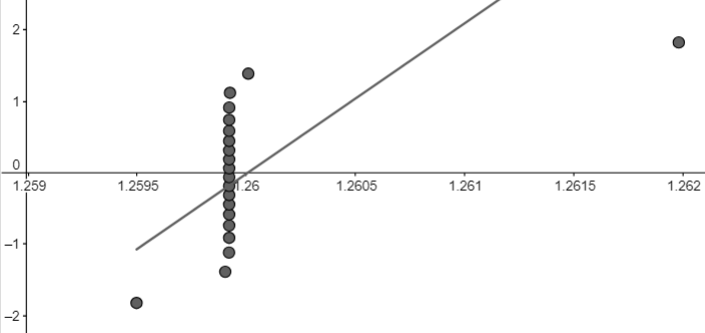
\includegraphics[width=0.68\linewidth]{images/plot.png}
	\caption{График}
	\label{fig:plot}
\end{figure}
\newpage

\section{Определение}
%Для любого $b_{0} > 0$
\begin{equation}
\sqrt[3]{2}= \underset{n\to \infty }{lim} \sqrt{1+b_{n}}
\end{equation}
где:   
\begin{equation}
b_{0} > 0,\ \hspace{15pt} b_{1}=\dfrac{1}{\sqrt{1+b_{0}^{2}}},\ \hspace{15pt} b_{2}=\frac{2\times b_{1}}{1+b_{1}}\times\frac{\sqrt{3}}{2}
\end{equation}
\begin{equation}
b_{3}=\dfrac{1}{\sqrt{1+b_{2}^{2}}},\ \hspace{15pt} b_{4}=\frac{2\times b_{3}}{1+b_{3}}\times\frac{\sqrt{3}}{2} \ ...
\end{equation}
\begin{equation}
b_{n+1}=\dfrac{1}{\sqrt{1+b_{n}^{2}}},\ \hspace{15pt} b_{n+2}=\frac{2\times b_{n+1}}{1+b_{n+1}}\times\frac{\sqrt{3}}{2}
\end{equation}
\\

\begin{center}
	Таким образом в пределе мы получим (см. Рис. \ref{fig:definition}) следующее:
\end{center}
\begin{equation}
d=\frac{a}{s}=\frac{1}{\sqrt{1+b^{2}}}
\end{equation}
\\
\begin{equation}
 b=g=\frac{2\times d}{1+d}\times\frac{\sqrt{3}}{2}
\end{equation}
\\
\begin{equation}
s=\dfrac{1}{d}=\sqrt[3]{2}
\end{equation}
\\
\begin{figure}[h]
	\centering
	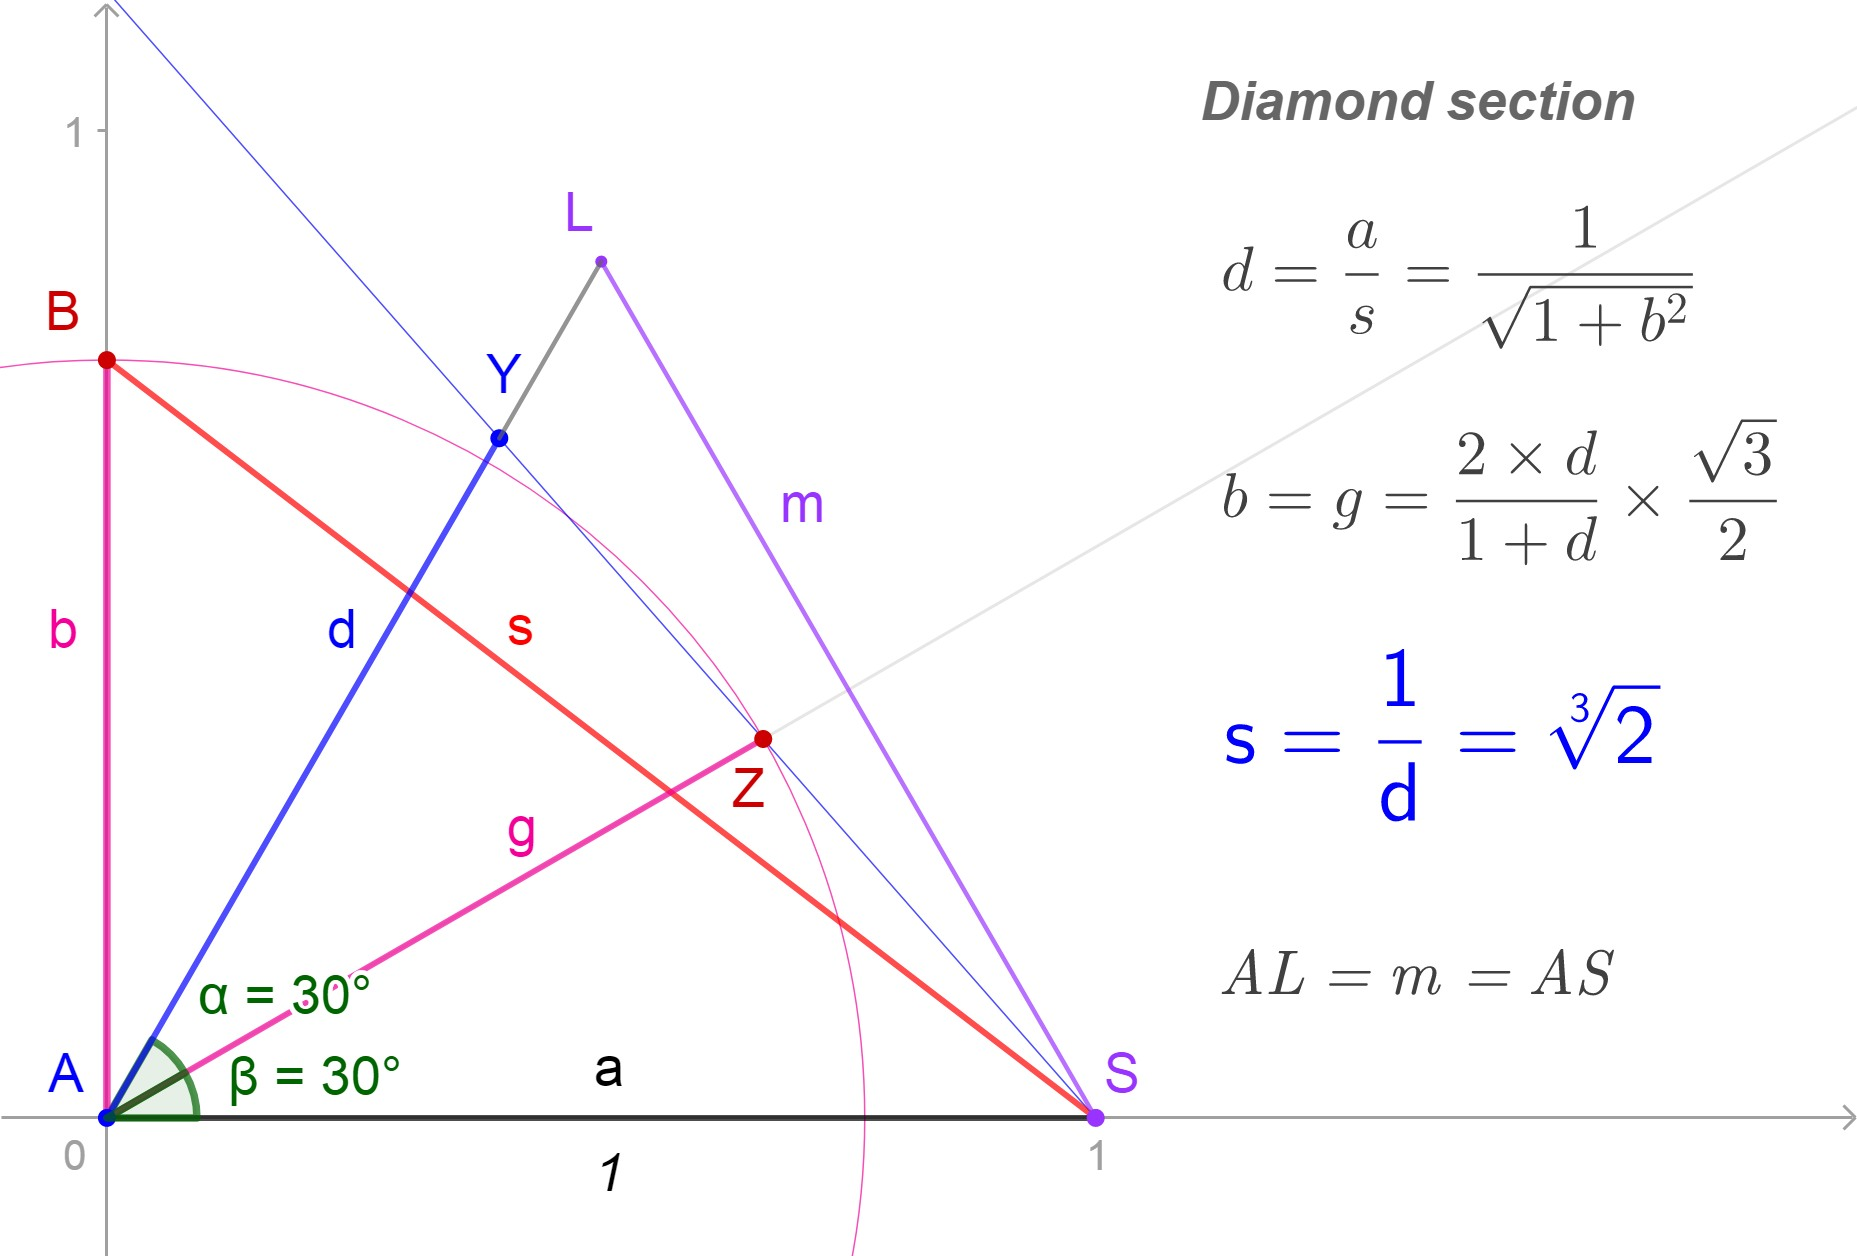
\includegraphics[width=0.7\linewidth]{images/ds_new_def.jpg}
	\caption{}
	\label{fig:definition}
\end{figure} \\

\begin{center}
	%\large{Diamond section of  $60 \degree$ angle = $\sqrt[3]{2}$ }
%\\
%\begin{equation}
%$\sqrt[3]{2}=\lim_{ n \to \infty } \sqrt{1^{2}+b_{n}^{2}}$; $b_{1}>0$; 
%\end{equation} 
%$\sqrt[3]{2}=\lim_{ n \to \infty\frac{1}s_{n}}$
\end{center}
\newpage
 
\section{Заключение}

%Мы построили геометрически\footnote{Используя только окружности и прямые линии т.е. циркулем и линейкой}, кубическое уравнение вида:
%\begin{equation}
%y=0.375x^{3}-0.5x^{2}+1.25x
%\end{equation}
%что ранее считалось невозможным.\\
 
Мы видели, что применяя определенную последовательность действий, возможно получить $\sqrt[3]{2}$ с любой, какой угодно заданной точностью. При этом мы используем только циркуль и неразмеченную линейку. Также мы ознакомились с  нетривиальным способом геометрических построений, который нигде до этого момента не упоминался.\\
%Можно ли считать задачу решенной?
% - надо бы спросить у Дельфийского оракула...



\begin{figure}[h]
	\centering
	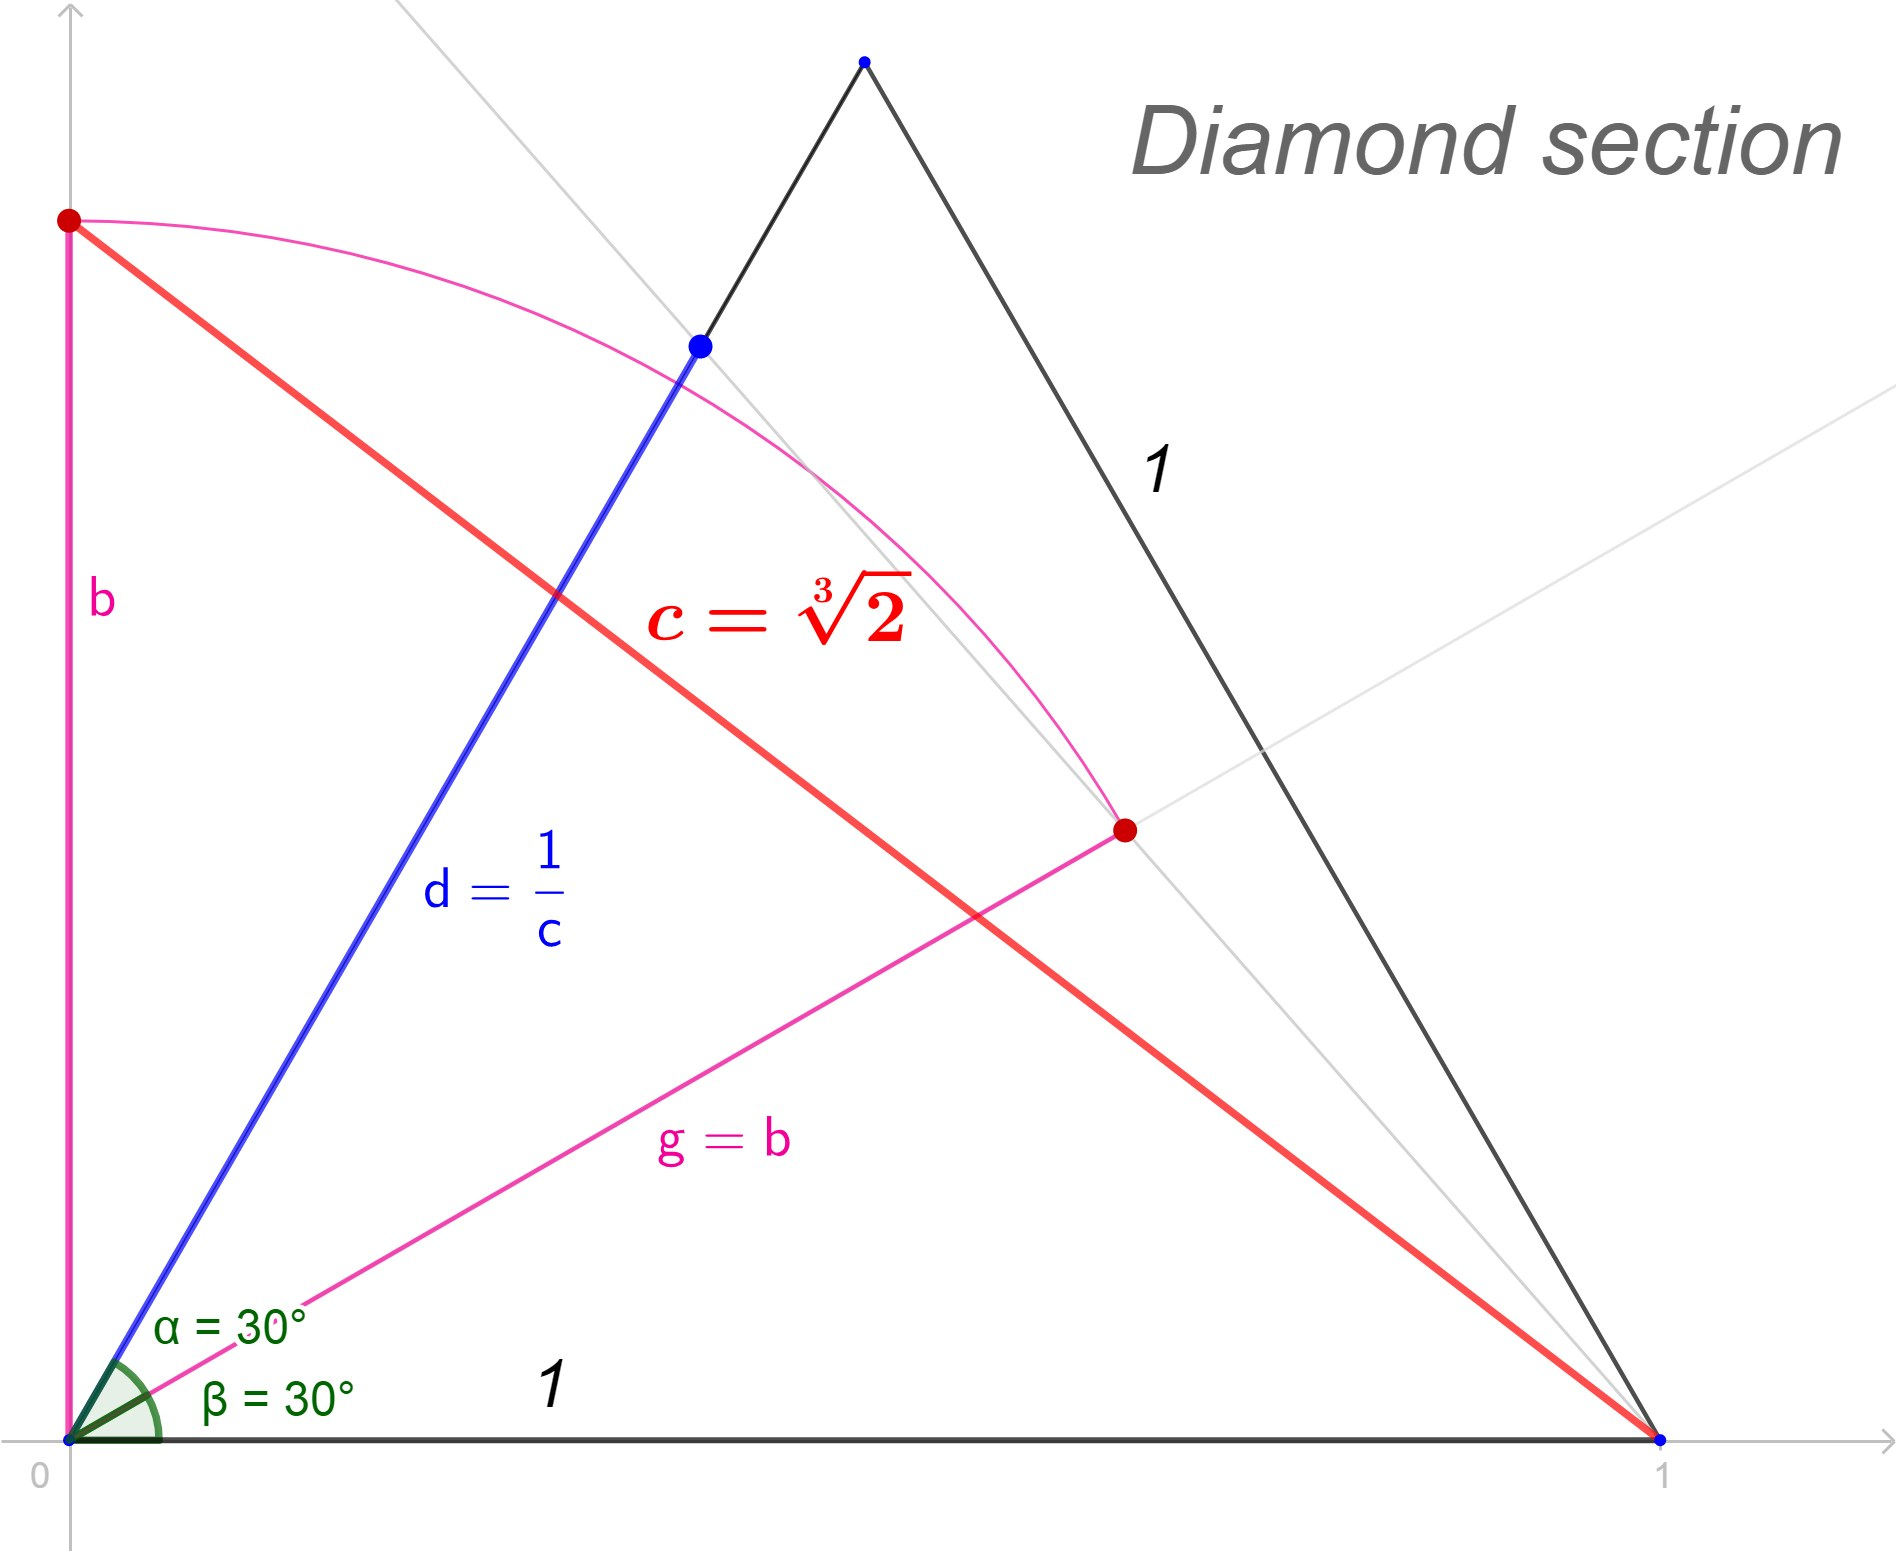
\includegraphics[width=0.6\linewidth]{images/ds_def.jpg}
	
	\label{fig:Diamond Section}
\end{figure}

\newpage

\section{Приложение}

Я нашел интересное свойство треугольника со сторонами: $a=1$; $b=\sqrt{\varphi-1}$; $c=\sqrt{\varphi}$\\
где $\varphi\approx 1.6180339887$ (см. Рис. \ref{fig:mytriangle})
\begin{figure}[h]
	\centering
	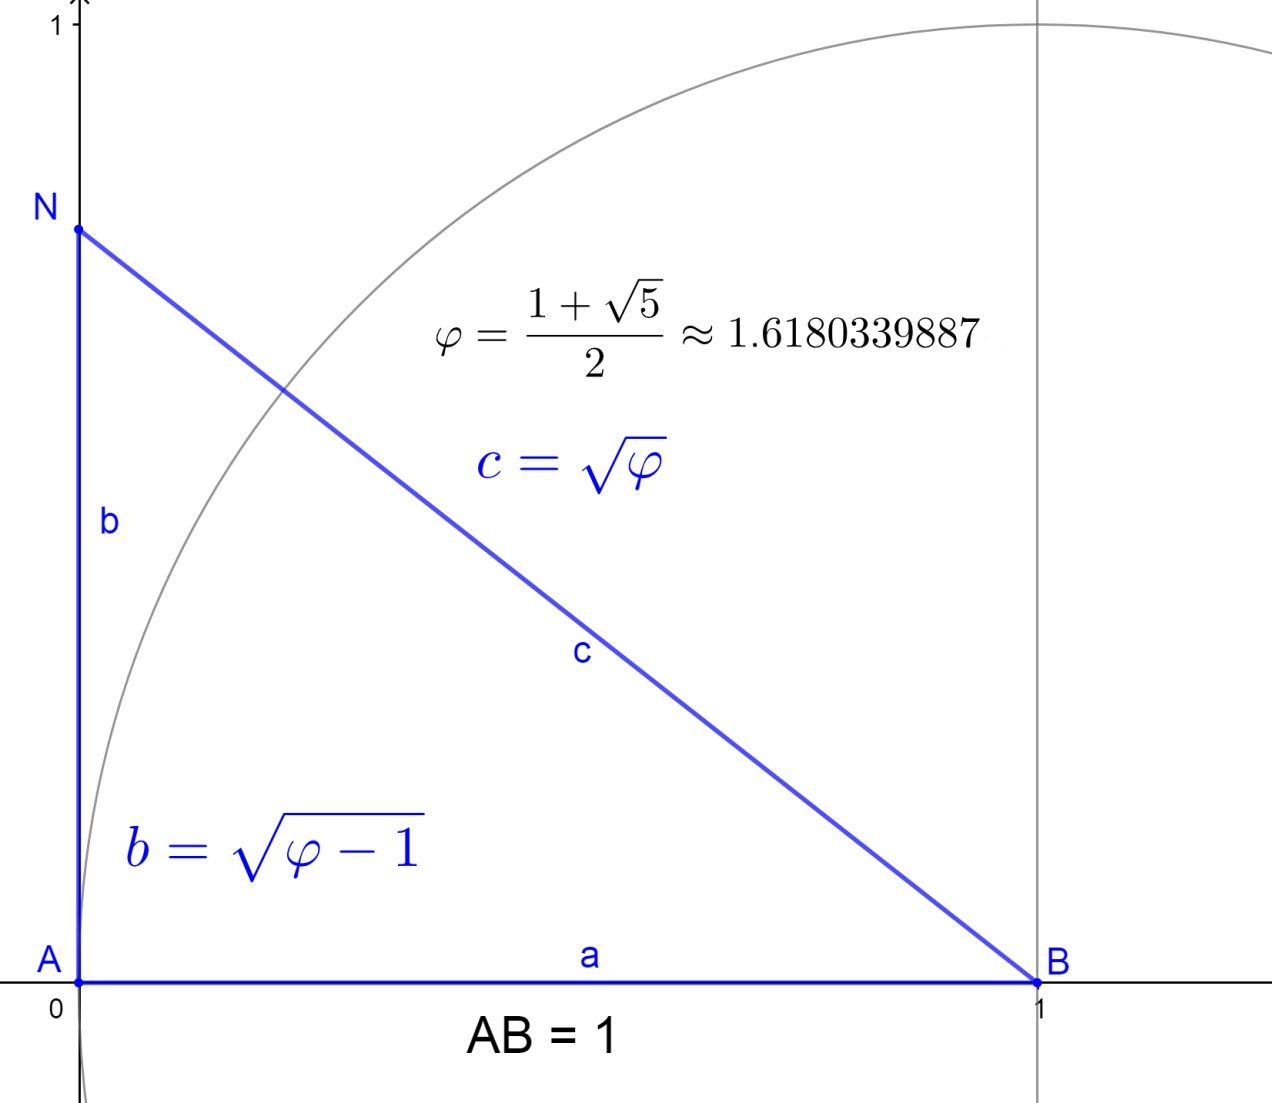
\includegraphics[width=0.7\linewidth]{images/my_triangle.jpg}
	\caption{Интересный треугольник}
	\label{fig:mytriangle}
\end{figure}

Если мы возьмем \textbf{произвольную} сторону $b$ для прямоугольного треугольника $a=1$, и рекурсивно применим следующее:
\begin{equation}
\dfrac{1}{\sqrt{a^2+b^2}} = b_{1}; \   \dfrac{1}{\sqrt{a^2+b_{1}^2}} = b_{2}; \   \dfrac{1}{\sqrt{a^2+b_{2}^2}}=b_{3}; \ ... \dfrac{1}{\sqrt{a^2+b_{n-1}^2}}=b_{n}
\end{equation} 
То после n-ного количества итераций мы получим следующие значения:
\begin{equation}
a=1;
\end{equation}
\\
\begin{equation}
b=\sqrt{\varphi-1}
\end{equation}
\\
\begin{equation}
c=\sqrt{\varphi}
\end{equation}
Следовательно наш треугольник с произвольно выбранной стороной $b$ стал равен треугольнику показанному на рис. \ref{fig:mytriangle}.
\\
Другими словами произвольно выбранная сторона $b$ стремится к $\sqrt{\varphi-1}$
\\
%Definition: \\
%\begin{equation}
%\sqrt{\varphi-1}=\lim_{n\to\infty}\dfrac{1}{d_{n}}; \      b>0; \   
%d_{1}=\dfrac{1}{\sqrt{1^{2}+b^{2}}}; \  \    %d_{2}=\dfrac{1}{\sqrt{{1^2+d_{1}^2}}}; \  ...\ %d_{n}=\dfrac{1}{\sqrt{{1^2+d_{n-1}^2}}}
%\end{equation}
%\begin{equation}
%\sqrt{\varphi}=\lim_{n\to\infty}\sqrt{d_{n}^2+1}; \      b>0; \   
%d_{1}=\dfrac{1}{\sqrt{1^{2}+b^{2}}}; \  \    %d_{2}=\dfrac{1}{d_{1}}; \  ...\ %d_{n}=\dfrac{1}{d_{n-1}};
%\end{equation}

%TODO: To construct the $\pi$ by using a compass and straightedge.\\
%next time 
 
\newpage


\begin{minipage}{0.8\textwidth}

\title{text}

	
\section{Ссылки}

%\large \textbf{Author:}

website: \url{ http://diamondsection.com} \\
e-mail: jobspace@yandex.com \\
github: \url{https://github.com/AlmasAskarbekov}

\section{Благодарность}
\url{https://geogebra.org}
\\

\end{minipage}
\vspace{365pt}
\hrule
\ 
\\
\emph{Keywords: Удвоение куба, античные задачи, Geometric problems of Antiquity, geometry, doubling the cube, the delians problem}




\begin{thebibliography}{5}
\bibitem{A}
\url{https://en.wikipedia.org/wiki/Doubling_the_cube}
\bibitem{B}
\url{https://oeis.org/A002580}
\end{thebibliography}

\vspace{465pt}
@misc{DiamondSection2018,
	author = {Almas Askarbekov},
	title = {Удвоение куба. Исследование},
	year = {2018},
	howpublished = {\url{https://github.com/DiamondSection/Doubling-the-cube-Solution_Latex}},
	note = {commit dbgsxxx}
}
%%%%%%Dedicated to Delos%%%%%%%% 
\end{document}